% mnras_template.tex 
%
% LaTeX template for creating an MNRAS paper
%
% v3.0 released 14 May 2015
% (version numbers match those of mnras.cls)
%
% Copyright (C) Royal Astronomical Society 2015
% Authors:
% Keith T. Smith (Royal Astronomical Society)

% Change log
%
% v3.0 May 2015
%    Renamed to match the new package name
%    Version number matches mnras.cls
%    A few minor tweaks to wording
% v1.0 September 2013
%    Beta testing only - never publicly released
%    First version: a simple (ish) template for creating an MNRAS paper

%%%%%%%%%%%%%%%%%%%%%%%%%%%%%%%%%%%%%%%%%%%%%%%%%%
% Basic setup. Most papers should leave these options alone.
\documentclass[fleqn,usenatbib]{mnras}

% MNRAS is set in Times font. If you don't have this installed (most LaTeX
% installations will be fine) or prefer the old Computer Modern fonts, comment
% out the following line
\usepackage{newtxtext,newtxmath}
% Depending on your LaTeX fonts installation, you might get better results with one of these:
%\usepackage{mathptmx}
%\usepackage{txfonts}

% Use vector fonts, so it zooms properly in on-screen viewing software
% Don't change these lines unless you know what you are doing
\usepackage[T1]{fontenc}

% Allow "Thomas van Noord" and "Simon de Laguarde" and alike to be sorted by "N" and "L" etc. in the bibliography.
% Write the name in the bibliography as "\VAN{Noord}{Van}{van} Noord, Thomas"
\DeclareRobustCommand{\VAN}[3]{#2}
\let\VANthebibliography\thebibliography
\def\thebibliography{\DeclareRobustCommand{\VAN}[3]{##3}\VANthebibliography}


%%%%% AUTHORS - PLACE YOUR OWN PACKAGES HERE %%%%%

% Only include extra packages if you really need them. Common packages are:
\usepackage{graphicx}	% Including figure files
\usepackage{amsmath}	% Advanced maths commands
\usepackage{amssymb}	% Extra maths symbols

%%%%%%%%%%%%%%%%%%%%%%%%%%%%%%%%%%%%%%%%%%%%%%%%%%

%%%%% AUTHORS - PLACE YOUR OWN COMMANDS HERE %%%%%

% Please keep new commands to a minimum, and use \newcommand not \def to avoid
% overwriting existing commands. Example:
%\newcommand{\pcm}{\,cm$^{-2}$}	% per cm-squared

%%%%%%%%%%%%%%%%%%%%%%%%%%%%%%%%%%%%%%%%%%%%%%%%%%

%%%%%%%%%%%%%%%%%%% TITLE PAGE %%%%%%%%%%%%%%%%%%%

% Title of the paper, and the short title which is used in the headers.
% Keep the title short and informative.
\title[Symmetry Energy Constraints from RSFs]{Resonant Shattering Flares as Multimessenger Probes of the Nuclear Symmetry Energy}

% The list of authors, and the short list which is used in the headers.
% If you need two or more lines of authors, add an extra line using \newauthor
\author[D. Neill et al.]{
Duncan Neill,$^{1}$\thanks{E-mail: dn431@bath.ac.uk}
William Newton,$^{2}$
David Tsang$^{1}$
\\
% List of institutions
$^{1}$Department of Physics, University of Bath, Claverton Down, Bath, BA1 1AL\\
$^{2}$Department of Physics and Astronomy, Texas A\&M University-Commerce, Commerce, TX, 75429-3011
}

% These dates will be filled out by the publisher
\date{Accepted XXX. Received YYY; in original form ZZZ}

% Enter the current year, for the copyright statements etc.
\pubyear{2015}

% Don't change these lines
\begin{document}
\label{firstpage}
\pagerange{\pageref{firstpage}--\pageref{lastpage}}
\maketitle

% Abstract of the paper
\begin{abstract}
The behaviour of the nuclear symmetry energy near saturation density is important for our understanding of dense nuclear matter. This density dependence can be parameterised by the nuclear symmetry energy and its derivatives evaluated at nuclear saturation density. In this work, we show that the core-crust interface mode of a neutron star is sensitive to these parameters, through the (density-weighted) shear-speed within the crust, which is in turn dependent on the symmetry energy profile of dense matter. We calculate the frequency at which the neutron star quadrupole ($\ell = 2$) crust-core interface mode must be driven by the tidal field of its binary partner to trigger a Resonant Shattering Flare (RSF). We demonstrate that coincident multimessenger timing of a RSF and gravitational wave chirp from a neutron star merger would enable us to place strong constraints on the symmetry energy parameters, competitive with those from current nuclear experiments.
\end{abstract}

% Select between one and six entries from the list of approved keywords.
% Don't make up new ones.
\begin{keywords}
dense matter -- stars: neutron -- stars: oscillations -- neutron star mergers -- gravitational waves -- equation of state
\end{keywords}

%%%%%%%%%%%%%%%%%%%%%%%%%%%%%%%%%%%%%%%%%%%%%%%%%%

%%%%%%%%%%%%%%%%% BODY OF PAPER %%%%%%%%%%%%%%%%%%

% \section{Introduction}

% This is a simple template for authors to write new MNRAS papers.
% See \texttt{mnras\_sample.tex} for a more complex example, and \texttt{mnras\_guide.tex}
% for a full user guide.

% All papers should start with an Introduction section, which sets the work
% in context, cites relevant earlier studies in the field by \citet{Fournier1901},
% and describes the problem the authors aim to solve \citep[e.g.][]{vanDijk1902}.
% Multiple citations can be joined in a simple way like \citet{deLaguarde1903, delaGuarde1904}.

% \section{Methods, Observations, Simulations etc.}

% Normally the next section describes the techniques the authors used.
% It is frequently split into subsections, such as Section~\ref{sec:maths} below.

% \subsection{Maths}
% \label{sec:maths} % used for referring to this section from elsewhere

% Simple mathematics can be inserted into the flow of the text e.g. $2\times3=6$
% or $v=220$\,km\,s$^{-1}$, but more complicated expressions should be entered
% as a numbered equation:

% \begin{align}
%     x=\frac{-b\pm\sqrt{b^2-4ac}}{2a}.
% 	\label{eq:quadratic}
% \end{align}

% Refer back to them as e.g. equation~(\ref{eq:quadratic}).

% \subsection{Figures and tables}

% Figures and tables should be placed at logical positions in the text. Don't
% worry about the exact layout, which will be handled by the publishers.

% Figures are referred to as e.g. Fig.~\ref{fig:example_figure}, and tables as
% e.g. Table~\ref{tab:example_table}.

% % Example figure
% \begin{figure}
% 	% To include a figure from a file named example.*
% 	% Allowable file formats are eps or ps if compiling using latex
% 	% or pdf, png, jpg if compiling using pdflatex
% 	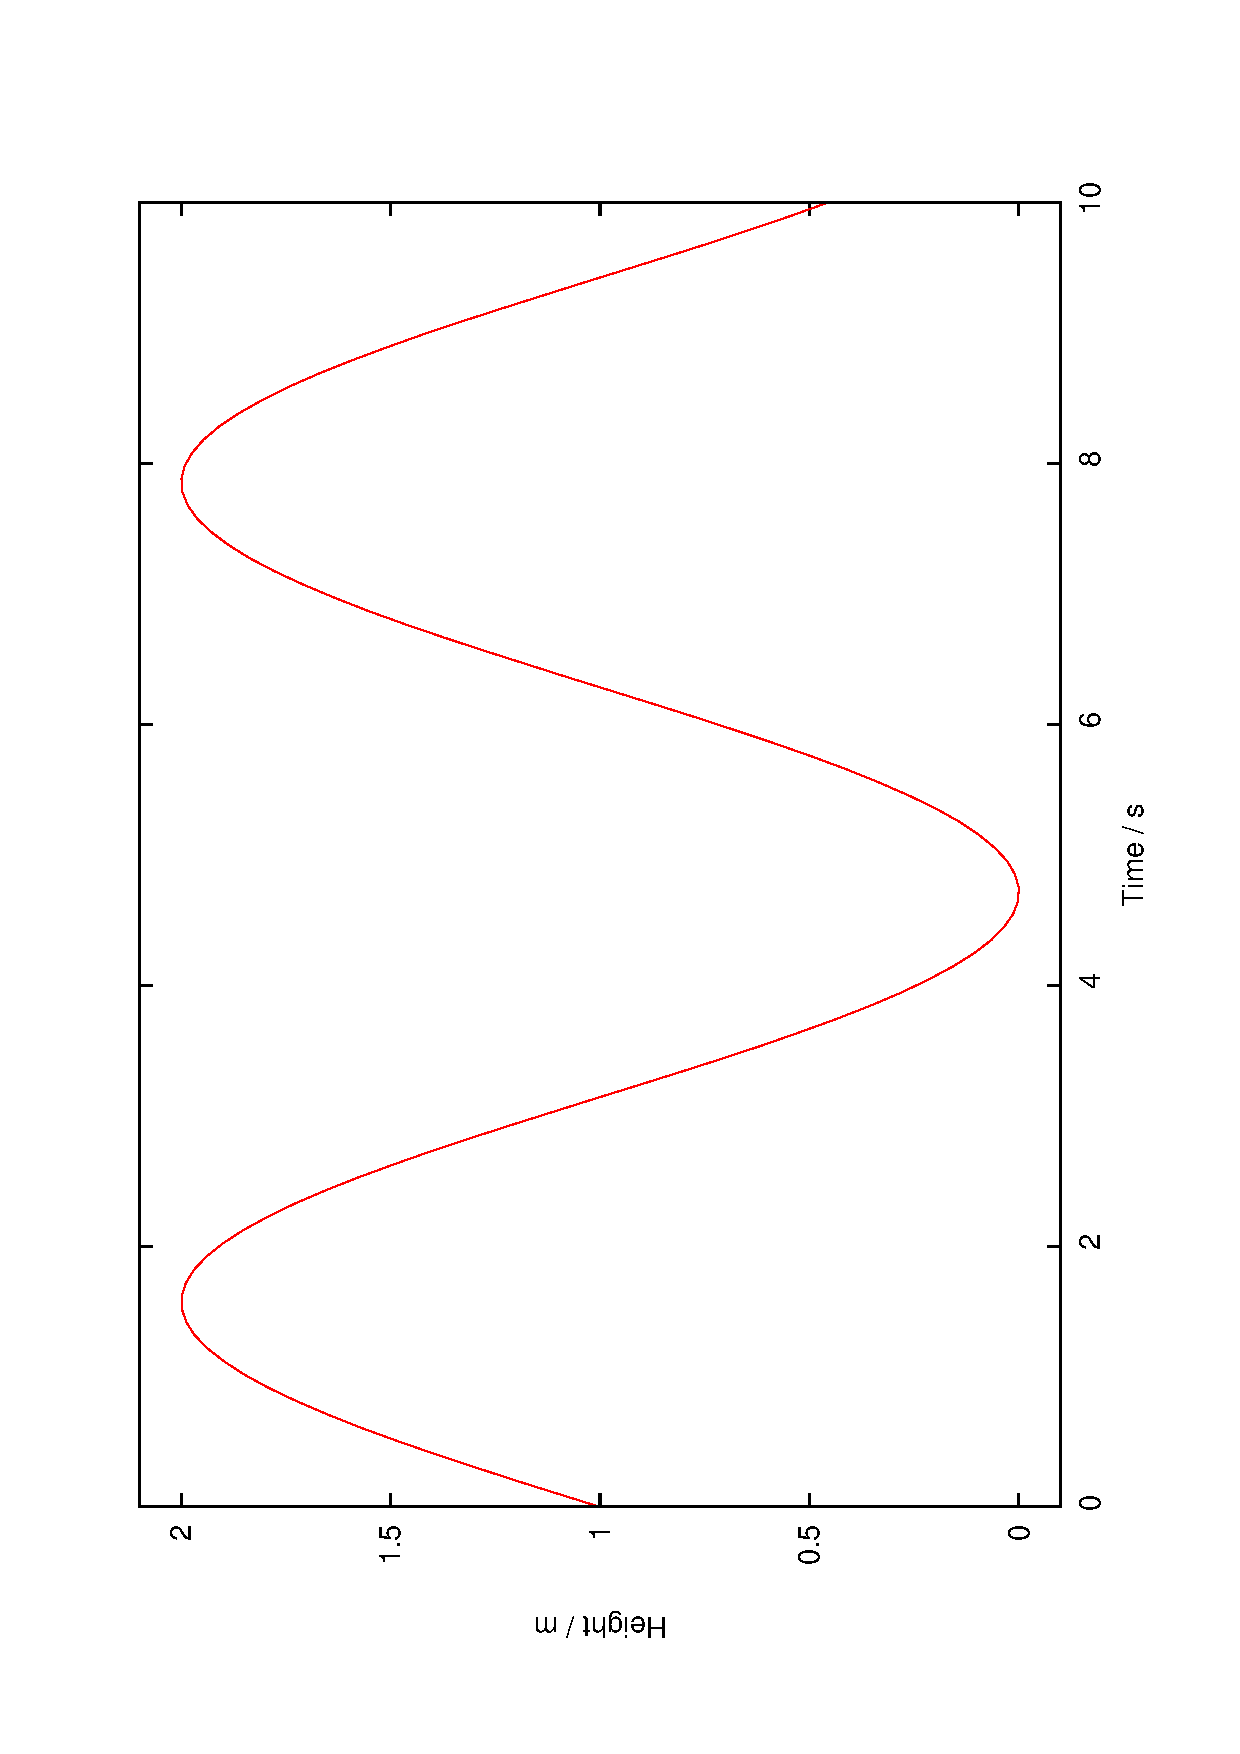
\includegraphics[width=\columnwidth]{example}
%     \caption{This is an example figure. Captions appear below each figure.
% 	Give enough detail for the reader to understand what they're looking at,
% 	but leave detailed discussion to the main body of the text.}
%     \label{fig:example_figure}
% \end{figure}

% % Example table
% \begin{table}
% 	\centering
% 	\caption{This is an example table. Captions appear above each table.
% 	Remember to define the quantities, symbols and units used.}
% 	\label{tab:example_table}
% 	\begin{tabular}{lccr} % four columns, alignment for each
% 		\hline
% 		A & B & C & D\\
% 		\hline
% 		1 & 2 & 3 & 4\\
% 		2 & 4 & 6 & 8\\
% 		3 & 5 & 7 & 9\\
% 		\hline
% 	\end{tabular}
% \end{table}


% \section{Conclusions}

% The last numbered section should briefly summarise what has been done, and describe
% the final conclusions which the authors draw from their work.


 
% The inclusion of a Data Availability Statement is a requirement for articles published in MNRAS. Data Availability Statements provide a standardised format for readers to understand the availability of data underlying the research results described in the article. The statement may refer to original data generated in the course of the study or to third-party data analysed in the article. The statement should describe and provide means of access, where possible, by linking to the data or providing the required accession numbers for the relevant databases or DOIs.


\section{Introduction}
\hspace{\parindent}
 
Neutron stars contain the most extreme matter in the universe. They act as natural laboratories to investigate nuclear physics, allowing us to study the physics of matter at nuclear densities. To investigate the internal structure of these compact stars we must probe them using observational phenomena.

Short gamma-ray bursts (SGRBs) \citep{kouveliotou1993identification,d2015short} likely originate from the merging of binary neutron stars \citep{eichler1989nucleosynthesis,fong2009hubble}. These bursts are characterised by a large peak in the gamma-ray count that lasts for $\sim 2$ second or less. Around $\sim3-10$\% of SGRBs are preceded by a `precursor' flare \citep{zhong2019precursors,troja2010precursors}. 
Precursor flares can be identified as a lower, separate peak in the gamma-ray count a short time ($\sim 0.1-5.0$ s) before the main peak \citep{zhong2019precursors}. 
Resonant Shattering Flares \citep{tsang2012resonant} are relatively isotropic, short ($\sim 0.1$s duration) gamma-ray flares that are triggered by a tidal resonance of the binary, and can appear as either precursor flares, or orphan flares if the main SGRB is beamed away from the observer. 



Recent observations of neutron star merger GW170817 \citep{abbott2017gw170817,goldstein2017ordinary} have begun a new era of multi-messenger astronomy involving gravitational waves and counterparts across the electromagnetic spectrum, allowing an unprecedented probe into the physics of binary neutron star mergers \citep[see e.g. ][ and references therein]{raithel2019constraints}. Here, we will show how multi-messenger coincident timing of a gravitational-wave chirp and the prompt-gamma ray emission from a Resonant Shattering Flare can be used to determine the frequency of a particular neutron star oscillation mode and hence constrain fundamental parameters in nuclear physics.


\subsection{Resonant Shattering Flares}
\hspace{\parindent}During the gravitational-wave induced inspiral of neutron star binaries, the normal modes of a neutron star can become excited by resonant tidal interactions with its binary partner. As the binary orbit shrinks, the frequency of the orbit (and hence the gravitational wave frequency) increases. When the orbital frequency sweeps through the appropriate resonance windows, the normal modes are excited, causing their oscillations to rapidly grow in magnitude \citep{tsang2012resonant, tsang2013shattering, lai1994resonant}.

If a resonant mode is sufficiently large to cause a deformation that exceeds the breaking strain in the neutron star crust, the crust will fracture, depositing seismic energy into the crust. One such mode is the quadrupole crust-core interface (i) mode. This mode is caused by the discontinuity in bulk material properties between the crust and core, and has a sufficient overlap with the tidal field \citep{tsang2012resonant} for the resonance to quickly deposit energy into the mode. The fractures and seismic waves continue to be driven until the crust reaches its elastic limit, causing it to shatter, scattering the seismic waves to high frequencies that are able to couple to the star's magnetic field, depositing energy into the magnetosphere and sparking a pair-photon fireball. Multiple colliding shells may be emitted over the course of the resonance window ($t_{\rm res} \sim 0.1$ seconds), leading to a single non-thermal burst with a duration of the resonance time, and the maximum luminosity determined by the surface magnetic field strength \citep{tsang2013shattering}.

For sufficiently strong surface magnetic field, these Resonant Shattering Flares (RSFs) can be detectable well beyond the Advanced LIGO horizon. Coincident timing of the RSF prompt emission and the gravitational-wave chirp provides a precise measurement of the resonant mode frequency. Therefore, by using a model of the crust and core with consistent nuclear physics to calculate the i-mode frequency, the parameters of that model could be restricted to ranges which results in mode frequencies that closely match the observed gravitational wave frequency during the RSF.  

In this paper, we will explore the implications of a coincident multi-messenger detection of an RSF on constraining fundamental nuclear physics parameters. In particular we will explore the relationship between the i-mode frequency, neutron star structure, and the nuclear symmetry energy parameters that determines the behaviour of matter near nuclear saturation density. 







\subsection{Nuclear Symmetry Energy and Neutron Star Structure}
\hspace{\parindent}The mode frequencies are dependent on the neutron star equation of state (EOS), the relationship between the energy density and pressure within the star, and the composition of the crust as a function of density. At low densities the EOS can be accurately calculated by using the properties of experimentally measured nuclei \citep{baym1971ground}. However, at the extreme densities found in neutron stars we must rely on nuclear models to calculate the EOS, with different models giving significantly different EOSs. The dominant uncertainty arises from a relative lack of experimental data that probes neutron-rich matter. This uncertainty is conveniently captured by the nuclear symmetry energy $E_{\rm sym}$ that encodes the average energy per nucleon required to convert symmetric nuclear matter (number of protons $Z$ = number of neutrons $N$) into pure neutron matter ($Z$=0). At nuclear saturation density (the density of nucleons in a nucleus) the symmetry energy can be parameterised by the coefficients of its density expansion, the first three of which are the magnitude of the symmetry energy at saturation density,
\begin{align}
J=E_{\rm sym}(n_0),    
\label{eq:sym_J}
\end{align}
\noindent its first derivative,
\begin{align}
L=3n_0\frac{\partial E_{\rm sym}(n_{\rm b})}{\partial n_{\rm b}}\biggr\rvert_{n_{\rm b}=n_0},  
\label{eq:sym_L}
\end{align}
\noindent and its second derivative
\begin{align}
K_{\rm sym}=9n_0^2\frac{\partial^2 E_{\rm sym}(n_{\rm b})}{\partial n_{\rm b}^2}\biggr\rvert_{n_{\rm b}=n_0},
\label{eq:sym_K}
\end{align}
\noindent where $n_0\approx 0.16$ fm$^{-3}$ is the nuclear saturation density and $n_{\rm b}$ is the baryon density.

\noindent These parameters have some simple physical implications. The magnitude of the symmetry energy $J$ controls the proton fraction at that density. The slope $L$ correlates with the pressure at that density, and $K_{\rm sym}$ controls the derivative of pressure, thus determining how rapidly the pressure increases as one moves away from saturation density, and plays an important role determining the stability of matter and its compressibility. Through these effects, neutron star structure and composition are sensitive to the symmetry energy and related nuclear observables \citep{Brown:2000aa, Horowitz:2001aa, Steiner:2008aa, Fattoyev:2018aa}, and astrophysical observations provide information on $E_{\rm sym}$ that complements nuclear experiment. Constraining the symmetry energy has been a priority in the field of nuclear physics over the past two decades \citep{Tsang:2012qy,Li:2014fj,Horowitz:2014aa}, and the burgeoning field of multimessenger astronomy provides exciting opportunities to synthesise astrophysical observation and nuclear experiment to learn more about the dense matter \citep{Tsang:2019ab}. Crust properties and their observational manifestations are particularly sensitive to the symmetry energy \citep{Newton:2013aaa}, including shear waves in the dense regions of the inner crust \citep{steiner2009constraints,Sotani2012a-crustosc,Sotani2013b-crustosc,Newton:2011crustosc}. RSFs are therefore a strong candidate to probe the symmetry energy \citep{tsang2012resonant,Newton:2013aaa}.

\section{Parameterised Neutron Star Equation of State and Composition}

\subsection{The Nuclear model} \label{sec:nuclear_model}

A consistent nuclear physics description of a neutron star requires an underlying nuclear model. We use an extended Skyrme mean field model for the uniform matter EOS \citep{holt2018universal}. Three parameters of the model affect only the pure neutron matter EOS, and can be written in terms of $J$, $L$ and $K_{\rm sym}$ \citep{newton2020nuclear,Balliet:2020aa}. Three degrees of freedom are required to give good fits to the predictions of chiral effective field theory calculations of the PNM EOS as well as some basic nuclear properties such as the masses and charge radii of doubly magic nuclei \cite{holt2018universal}. We can therefore take a range for $J$, $L$ and $K_{\rm sym}$ and systematically generate a set of extended-Skyrme models and resulting crust and core equations of state.

We explore the distributions of $i$-mode frequencies on three sets of symmetry energy parameters.

\begin{figure}
\centering
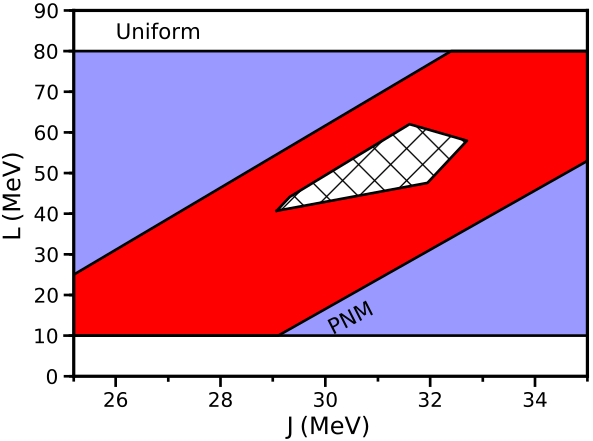
\includegraphics[width=0.45\textwidth,angle=0]{JLsim-Ranges_v2.png}
\caption{The ranges use for the first two symmetry energy parameters $J$ and $L$. Both our Uniform and MSL0 sets cover the space colored in blue from $L$=10 to 80 MeV and $J$=25 to 35 MeV. The PNM set covers the region in red uniformly. Also picture is the region in the intersection of a number of nuclear experimental constraints, taken from \citet{lattimer2013constraining}.}
\label{fig:JLRanges}
\end{figure}

(i) Our most conservative range of EOSs uses symmetry energy parameters uniformly distributed over the ranges $25\leq J\leq 35$ MeV, $10\leq L\leq 80$ MeV, and $-200\leq K_{\rm sym}\leq 40$ MeV. These ranges were chosen to cover the ranges predicted by other works \citep{liu2010nuclear,tsang2012constraints,lattimer2013constraining}. This will be referred to as our ``uniform'' distribution, and is shown in the shaded blue region of figure~\ref{fig:JLRanges}.

(ii) The properties of pure neutron matter are the most important ingredient in the crust EOS, so relevant constraints for neutron stars comes from pure neutron matter theory. Great strides have been made in modeling pure neutron matter from first principles, particularly using chiral effective field theory. Based on this and some general consideration from Fermi liquid theory \citep{holt2018universal}, we defined a conservative range of symmetry energy parameter space in which all $ab-initio$ predictions of the PNM EOS lie. Details of the ranges used are given in \citet{newton2020nuclear}. The range in $J$-$L$ space is shown as the red shaded region in figure~\ref{fig:JLRanges}. This will be referred to as our ``PNM'' distribution.

(iii) In many Skyrme models, such as Sly4 \citep{chabanat1998skyrme} and SkI6 \citep{reinhard1995nuclear,nazarewicz1996structure}, there are only two parameters that control the PNM EOS alone, and therefore $K_{\rm sym}$ is not a free parameter. In order to disentangle the effects of the symmetry energy parameters on the $i$-mode frequencies, it will be useful examine models with only $J$ and $L$ as free parameters. We take the dependence of $K_{\rm sym}$ from the MSL0 interaction \citep{chen2009higher}, has previously been used to extract symmetry energy constraints from nuclear experiment. In that model, $K_{\rm sym}$ is related to $J$ and $L$ by \citep{newton2020nuclear}
\begin{align}
K_{\rm sym}=3.71L-11.13J+11.93\; \rm{MeV},
\end{align}
\noindent which restricts us to a single plane in the $J$,$L$,$K_{\rm sym}$ parameter space. We will refer to this as our ``MSL0'' distribution. Note that there is nothing physically special about this particular choice of relation between the symmetry energy parameters.
It allows us to assess the importance of uncertainty in $K_{\rm sym}$.

We show the regions of $J$-$L$ space we sample for each of the three distributions in figure~\ref{fig:JLRanges}. The regions we cover encompass a number of nuclear experimental constraints, the intersection of which is also shown as the white hatched region \cite{lattimer2013constraining}.  

\subsection{The crust model}

To calculate the crust composition and EOS, we use our sets of extended Skyrme models in a compressible liquid drop model (CLDM) \citep{Newton:2013aa,Balliet:2020aa}. The model assumes a lattice consisting a single species of nucleus immersed in a neutron gas in a repeating unit cell (the Wigner-Seitz approximation). By minimising the energy of the unit cell with respect to the physical parameters of the box - the neutron gas density $n_{\rm n}$, the cell radius $r_{\rm c}$, and the mass and charge number of the nuclear cluster $A,Z$ - we obtain the ground state composition and EOS of the crust at a given density. We can then calculate quantities required to model the normal modes in the crust, for example the shear modulus and frozen-composition adiabatic index as a function of baryon density $n_{\rm b}$ \citep{strohmayer1991shear,Chugunov:2010aa}. 

%\begin{align}
%\mu=\frac{0.1106}{1+17810\left(\frac{ak_bT}{\left(Ze\right)^2}\right)^2}%\frac{n_i\left(Ze\right)^2}{a},
%\label{eq:mu_1991}
%\end{align}

The shear modulus in the crust is given by 
\begin{align}
\mu=\frac{0.1106}{1+17810\left(\frac{ak_bT}{\left(Ze\right)^2}\right)^2}\frac{n_i\left(Ze\right)^2}{a},
\label{eq:mu_1991}
\end{align}
\noindent where $T$ is the temperature, $n_i$ is the ion density, $Z$ is the proton number of the nuclei, and 
\begin{align}
a=\left(\frac{3}{4\pi n_i}\right)^{\frac{1}{3}}.
\label{eq:mu_1991_a}
\end{align}

We conduct calculations at zero temperature. The ion number density can be written in terms of the fraction of nucleons in the neutron gas $X_{\rm n}$ through the relation \citep{Newton:2013aa}

\begin{equation}
    X_{\rm N} = 1 - X_{\rm n} = \frac{n_{\rm i}}{n_b}A
    \label{eq:neutrons_ions}
\end{equation}

\noindent where $X_{\rm N}$ is the fraction of nucleons in the nucleus. 
We can therefore re-write the shear modulus as a function of $X_{\rm n}$ (at zero temperature) as \citep{Steiner:2008aa,Newton:2011crustosc}
\begin{equation}
	\mu = 0.1106 \left(\frac{4\pi}{3}\right)^{1/3} A^{-4/3} n_{\rm b}^{4/3} (1-X_{\rm n})^{4/3} (Ze)^2,
	\label{eq:altmu}
\end{equation}

The adiabatic index at constant composition is given by

\begin{equation} \label{eq:adiabatic_index}
\Gamma_{\rm 1} = \frac{n_{\rm b}}{P} \frac{dP}{dn_{\rm b}}\bigg|_{\rm constant \; composition} =  \frac{n_{\rm b}}{P} \bigg[\frac{dP_n}{dn_{\rm n}} +  x \frac{dP_e}{dn_{\rm e}}  \bigg]
\end{equation}

\noindent where $x$ is the average proton fraction and $P$ the total pressure. $P_{\rm n,e}$ are the pressures and $n_{\rm n,e}$ the number densities of dripped neutrons and electrons respectively.


\subsection{The core model}

The Skyrme model is designed to describe nuclear interactions around nuclear saturation density. As one moves into the neutron star core, the increasing importance of relativistic effects, the possible appearance of hyperons at supersaturation density, and the likely transition from nucleonic to quark degrees of freedom in the inner core mean the model is not suited to describe matter beyond about twice saturation density, and the symmetry energy loses its physical meaning. In order to explore the symmetry energy effects on RSFs, we do need to control the core EOS. We use the piecewise polytrope method \citep{Read:2009aa, Read:2009ab, Steiner:2010aa, Steiner:2013aa, Ozel:2009aa, Ozel:2010aa, Ozel:2016aa}: we fit two polytropes at supersaturation densities, one at a density of $n_1$=1.5$n_0$ and one at $n_2$=2.7$n_0$, as detailed in \cite{Newton:2018aa}. We then have three regions of the star: the crust and outer core, in which the pressure and energy density are given by the Skyrme EOS, and the two polytropic regions in which the pressures are given by

\begin{align}
\nonumber P = P_{\rm Skyrme} & \;\;\;\;\; n<n_1 \\
\nonumber P_1 = K_1 n^{\gamma_1}  & \;\;\;\;\;n_1 <n<n_2  \\
P_2 = K_2 n^{\gamma_2} & \;\;\;\;\;  n_2 < n
\end{align}

%\begin{align}\nonumber
%K_1 n_1^{\Gamma_1} &= P_{\rm Skyrme}   \\
%K_2 n_2^{\Gamma_2} &= K_1 n_1^{\Gamma_1} 
%\end{align}

\noindent where continuity of pressure determines the constants $K_1$ and $K_2$. The energy density in the three density regions is obtained by integrating the first law of thermodynamics:

\begin{equation}
\epsilon_i = (1+a_i)n + \frac{K_i n^{\gamma_i}}{\gamma_1 -1}; \;\;\;\;\;\;\; a_i = \frac{\epsilon_{i-1} (n_i)}{n_i} - \frac{K_i n^{\gamma_i - 1}}{\gamma_i -1} - 1
\end{equation}

\noindent where $a_i$ are constants of integration, $i$=\{1,2\} and the subscript 0 labels the Skyrme EOS.

The speed of sound is 

\begin{equation}
\frac{c_{\rm s,i}(n)}{c} = \bigg( \frac{\gamma_i P}{P + \epsilon}\bigg)^{1/2}
\end{equation}

In the eventuality that the EOS becomes acausal at a given density $n_{\rm acausal}$, we transition to a causal EOS:

\begin{equation}
P_{\rm causal} = \epsilon = bn^{1/3} \;\;\;\;\;  n_{\rm acausal} < n
\end{equation}

\noindent where $\epsilon$ is the energy density, $b$ is a constant given by

\begin{equation} 
b = \frac{1+a}{n_{\rm acausal}} + K \frac{n_{\rm acausal}^{\gamma-2}}{\gamma-1}
\end{equation}

\noindent and $a$ is either $a_1$ or $a_2$ depending on which region the EOS becomes acausal in.

Each equation of state generated is characterised by 5 parameters: the three symmetry energy coefficients $J$, $L$ and $K_{\rm sym}$ for the Skyrme-EOS, and the polytropic parameters $\gamma_1$ and $\gamma_2$. $\gamma_2$, which controls the high density part of the EOS, can be tuned to give a desired maximum mass. $\gamma_1$, which controls the EOS at intermediate densities in the core, can be tuned to give a particular moment of inertia of a 1.4$M_{\odot}$ star $I_{1.4}$ while keeping the other parameters fixed. We can thus parametrise each EOS by $J$, $L$, $K_{\rm sym}$, $I_{1.4}$ and $M_{\rm max}$.

The $i$-mode frequency is relatively insensitive to the high density EOS, and so in this work we fix the high density degrees of freedom $I_{1.4}$ and $M_{\rm max}$. We choose to fix $M_{\rm max}$ at 2.2$M_{\odot}$, comfortably above the maximum accurately measured pulsar mass \citep{cromartie2020relativistic} and consistent with maximum masses inferred from modeling of the binary neutron star merger resulting in GW170817. For $I_{1.4}$, for each EOS we take the average of the maximum and minimum possible value of the moment of inertia of a 1.4$M_{\odot}$ star.



\begin{figure}
\centering
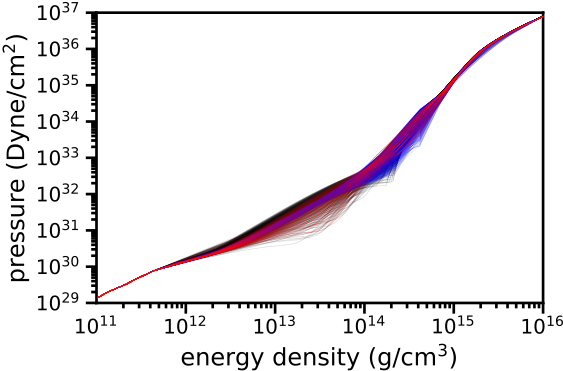
\includegraphics[width=0.45\textwidth,angle=0]{EoSs_lines.png}
\caption{The equations of state used in this work. The different colours are for the three different sets of symmetry energy parameters we have used, with the black being for weakly constrained parameters, blue for parameters constrained by nuclear matter theory, and red for $K_{\rm sym}$ having a MSL0-like dependence on $J$ and $L$.}
\label{fig:EoSs}
\end{figure}

The resultant EOSs are shown in Figure \ref{fig:EoSs}, and are used, along with the Tolman-Oppenheimer-Volkoff equations \citep{oppenheimer1939massive,tolman1939static}, to determine the grid of stellar models for which the i-mode frequencies are calculated. 


\section{Calculation of the Normal Modes}
\hspace{\parindent}We calculate the frequencies and radial/transverse displacements of the modes of a neutron star by linearly perturbing the equations defining the equilibrium state of neutron star matter. We assume that the binary lifetime is much larger than the spin-down and cooling times of the individual neutron stars, and so we may ignore rotation and high-temperature effects. We will also assume that the frequencies of the modes that we are interested in ($\sim 10 - 100$ Hz) result in oscillations that are significantly faster than the beta-equilibrium timescale. Therefore, weak-interactions do not have time to change the composition of a displaced mass element to more closely match the local composition.





\subsection{Basic Equations}
\hspace{\parindent}To construct a 2-component neutron star model (consisting of a solid crust and fluid core) we follow \citet{mcdermott1988nonradial}, beginning with the mass continuity equation, momentum conservation equation, and Poisson's equation:

\begin{align}
\frac{\partial\rho}{\partial t}+\nabla\cdot(\rho v)=0,
\label{eq:continuity_eqn}
\end{align}
\begin{align}
\frac{\partial v}{\partial t}=(v\cdot \nabla)v=\frac{1}{\rho}\nabla\cdot\sigma-\nabla\Phi,
\label{eq:momentum_eqn}
\end{align}
\begin{align}
\nabla^2\Phi=4\pi G\rho,
\label{eq:Poisson_eqn}
\end{align}
\noindent where $\rho$ is the energy density, $v$ is the velocity of the matter, $\sigma$ is the stress tensor, and $\Phi$ is the gravitational potential. By combining the linear perturbations of these equations, and taking the Cowling approximation by ignoring perturbations of the gravitational potential \citep{cowling1941non}, we obtain the wave equation
\begin{align}\nonumber
&&\omega^2u=-\nabla\left(\frac{\Gamma_1 p}{\rho}\nabla\cdot u\right)-\nabla\left(\frac{1}{\rho}u\cdot\nabla p\right)-\hat{r}A\frac{\Gamma_1 p}{\rho}\nabla\cdot u\\\nonumber
&&+\frac{1}{\rho}\biggr(\nabla\left(\frac{2}{3}\mu\nabla\cdot u\right)-\left(\nabla\mu\cdot\nabla\right)u-\nabla\left(u\cdot\nabla\mu\right)\\
&&+\left(u\cdot\nabla\right)\nabla\mu-\mu\left(\nabla^2 u+\nabla\left(\nabla\cdot u\right)\right)\biggr),
\label{eq:wave_eqn}
\end{align}
where $u(x,t)$ is the Lagrangian displacement,
\begin{align}
A=\frac{1}{\rho}\frac{d\rho}{dr}-\frac{1}{\Gamma_1P}\frac{dP}{dr}
\label{eq:schwartz_descrim}
\end{align}
\noindent is the Schwarzschild discriminant, and $\Gamma_1$ is the adiabatic index defined in equation \ref{eq:adiabatic_index}. The non-diagonal terms of the stress tensor are given by $\sigma_{ij} = \mu \nabla_i u_j$, assuming the isotropic shear modulus $\mu$ from equation~\ref{eq:altmu}.



Taking the perturbations to have time dependence of the form $e^{i\omega t}$, where $\omega$ is the mode frequency, we have 
\begin{align}
u(x,t)=\xi(x)e^{i\omega t}.
\label{eq:time_seperation}
\end{align}
\noindent In spherical coordinates this can be further separated into radial and transverse components:
\begin{align}
\xi_r=U(r)Y_{lm},\;\;\;\xi_{\theta}=V(r)\frac{\partial Y_{lm}}{\partial\theta},\;\;\;\xi_{\phi}=\frac{V(r)}{\sin(\theta)}\frac{\partial Y_{lm}}{\partial\phi},
\label{eq:xi_seperation}
\end{align}
\noindent where $U(r)$ is the radial displacement, $V(r)$ is the transverse displacement, and $Y_{lm}$ are the spherical harmonics.

By using the separation of variables given in equations \ref{eq:time_seperation} and \ref{eq:xi_seperation}, the wave equation can be rewritten in terms of $U$ and $V$:\footnote{The version of equation \ref{eq:Ueqn} in \citet{mcdermott1988nonradial} has a typographical error.} 
\begin{align}\nonumber
&&\rho\omega^2U=\rho\frac{d\hat{\chi}}{dr}-A\Gamma_1 p\hat{\alpha}-\frac{d}{dr}\left(\frac{1}{3}\mu\hat{\alpha}\right)+\frac{d\mu}{dr}\left(\hat{\alpha}-2\frac{dU}{dr}\right)\\
&&-\mu\left(\frac{1}{r^2}\frac{d}{dr}\left( r^2\frac{dU}{dr}\right)-\frac{\ell(\ell+1)}{r^2}U+\frac{2\ell(\ell+1)}{r^2}V-\frac{2}{r^2}U\right),
\label{eq:Ueqn}
\end{align}
\begin{align}\nonumber
&&\rho\omega^2V=\rho\frac{\hat{\chi}}{r}-\frac{1}{3}\frac{\mu\hat{\alpha}}{r}-\frac{d\mu}{dr}\left(\frac{dV}{dr}-\frac{V}{r}+\frac{U}{r}\right)\\
&&-\mu\left(\frac{1}{r^2}\frac{d}{dr}\left(r^2\frac{dV}{dr}\right)-\frac{\ell(\ell+1)}{r^2}V+\frac{2}{r^2}U\right),
\label{eq:Veqn}
\end{align}
% \begin{align}
% \frac{1}{r^2}\frac{d}{dr}\left(r^2\frac{d\hat{\Phi}'}{dr}\right)-\frac{\ell(\ell+1)}{r^2}\hat{\Phi}'=4\pi G\left(U\frac{d\rho}{dr}+\hat{\alpha}\rho\right),
% \label{eq:Phihat_eqn}
% \end{align}
\noindent where:\footnote{The version of equation \ref{eq:chihat} in \citet{mcdermott1988nonradial} has a typographical error.}
\begin{align}
\hat{\alpha}=\frac{1}{r^2}\frac{d}{dr}(r^2U)-\frac{\ell(\ell+1)}{r}V,
\label{eq:alphahat}
\end{align}
\begin{align}
\hat{\chi}=-\frac{\Gamma_1p}{\rho}\hat{\alpha}-\frac{1}{\rho}\frac{\partial p}{\partial r}U.
\label{eq:chihat}
\end{align}
\noindent In the crust these equations can be solved as a set of four first-order differential equations, whereas in the core these equations are simplified by the requirement that $\mu=0$, resulting in two first-order differential equations.

In this work we have applied Newtonian perturbations to a relativistic equilibrium stellar structure, resulting in a hybrid model. In order for this model to be usable, the modes must be orthogonal such that any perturbation can be expressed as a unique linear combination of the modes. The eigenfunction and eigenvalue of any mode can be defined in relation to the oscillation operator, $\mathcal{H}$, as shown by \citet{reisenegger1994multipole}:
\begin{align}
\mathcal{H}\xi=-\omega^2\xi.
\end{align}
\noindent Newtonian perturbations will only result in orthogonal modes if $\mathcal{H}$ is Hermitian with respect to the inner product of two vector fields (any two displacements of matter within the star), ie:
\begin{align}
\int_*\rho_0(r)\zeta^*(x)\cdot\mathcal{H}\Psi(x)d^3x=\int_*\rho_0(r)\mathcal{H}\zeta^*(x)\cdot\Psi(x)d^3x.
\end{align}
\noindent For a Newtonian stellar model the oscillation operator is Hermitian, and therefore applying Newtonian perturbations results in orthogonal modes. 

For a relativistic stellar model, the oscillation operator is not Hermitian. However, this does not pose a problem for a relativistic perturbation approach \citep[see e.g. ][]{yoshida2002nonradial} because their eigenfrequencies are complex numbers, with the imaginary component arising from the damping of the mode due to the emission of gravitational waves. This imaginary component cancels out the deviation from orthogonality that arises from $\mathcal{H}$ not being Hermitian, and so relativistic perturbations can be applied to a relativistic stellar model to obtain orthogonal modes.

The hybrid model we have adopted can cause problems, because the stellar model does not give a Hermitian oscillation operator and the eigenfrequencies of Newtonian oscillations do not have the imaginary component required to cancel out the modes' deviation from orthogonality. To fix this, we follow \citet{reisenegger1994multipole} and define the local acceleration due to gravity within the star as
\begin{align}
g=-\frac{1}{\rho}\frac{dP}{dr}.
\label{eq:rel_grav}
\end{align}
\noindent This form for the gravity makes the oscillation operator Hermitian within the relativistic model, and therefore we can apply Newtonian perturbations to this modified relativistic star to obtain orthogonal modes. %The change to the gravity somewhat changes the properties of the modes, but only to a small degree.










%Explain how we determine where Rcc is?

At the boundary between the solid crust and the fluid core, there are three jump conditions that must be satisfied:\footnote{The version of the left-hand side of equation \ref{eq:jump2} in \citet{mcdermott1988nonradial} has a typographical error.}
\begin{align}
U\rvert_{r=R_{\rm cc}^{+}}=U\rvert_{r=R_{\rm cc}^{-}},
\label{eq:jump1}
\end{align}
\begin{align}
\frac{1}{p}\left(\lambda\hat{\alpha}+2\mu\frac{dU}{dr}\right)\biggr\rvert_{r=R_{\rm cc}^{+}}=\tilde{V}\left(\frac{U}{r}-\frac{\omega^2V}{g}\right)\biggr\rvert_{r=R_{\rm cc}^{-}},
\label{eq:jump2}
\end{align}
\begin{align}
\frac{\mu}{p}\left(\frac{dV}{dr}-\frac{V}{r}+\frac{U}{r}\right)\biggr\rvert_{r=R_{\rm cc}^{+}}=0,
\label{eq:jump3}
\end{align}
\noindent where 
\begin{align}
\tilde{V}=-\frac{d\ln\left(P\right)}{d\ln\left(r\right)}=\frac{\rho g r}{p},
\end{align}
\begin{align}
\lambda=\Gamma_1P-\frac{2}{3}\mu
\end{align}
\noindent is the Lam\'e coefficient, 
\begin{align}
M_r=4\pi\int^r_0 r'^2\rho(r')dr'
\label{eq:mass_r}
\end{align}
\noindent is the mass contained within radius $r$, and $r=R_{\rm cc}^{+}$ ($r=R_{\rm cc}^{-}$) indicates that the value is evaluated at the boundary when approached from the crust (core) of the star. The three conditions require different properties to be continuous across the crust-core boundary. The first is for the radial displacement, the second is for the pressure, and the third is for the traction (which must be zero in the fluid core). The first two jump conditions can be combined in order to cancel out the arbitrary magnitude of $U$ and $V$ (which is different in the crust and the core), giving us
\begin{align}
\frac{r}{p}\frac{\left(\lambda\hat{\alpha}+2\mu\frac{dU}{dr}\right)}{U}\biggr\rvert_{r=R_{\rm cc}^{+}}=\tilde{V}\left(1-\frac{\sigma^2r}{g}\frac{V}{U}\right)\biggr\rvert_{r=R_{\rm cc}^{-}}.
\label{eq:jump2/1}
\end{align}
\noindent This leaves us with two jump conditions, equations \ref{eq:jump3} and \ref{eq:jump2/1}, and two eigenvalues, $\Omega$ and $V(R_*)$.


Every mode must satisfy the boundary conditions at the centre and surface of the star. The conditions at the surface are based on the requirement that the Lagrangian pressure perturbation goes to zero at the surface:
\begin{align}
\frac{1}{p}\left(\lambda\hat{\alpha}+2\mu\frac{dU}{dr}\right)\biggr\rvert_{r=R_{*}}=\tilde{V}\left(\frac{\tilde{V}-c_1\Omega^2-4+\tilde{U}}{\frac{\ell(\ell+1)}{c_1\Omega^2}-\tilde{V}}+1\right)\frac{U}{r}\biggr\rvert_{r=R_{*}},
\label{eq:surface_boundary_modified_1}
\end{align}
\begin{align}
\frac{\mu}{p}\left(\frac{dV}{dr}-\frac{V}{r}+\frac{U}{r}\right)\biggr\rvert_{r=R_{*}}=0,
\label{eq:surface_boundary_modified_2}
\end{align}
\noindent where every quantity is evaluated at the surface of the star ($r=R_*$), and 
\begin{align}\nonumber
\tilde{U}=\frac{d\ln\left(M_r\right)}{d\ln\left(r\right)}=4\pi r^2\rho\frac{r}{M_r},\;\;\;c_1=\left(\frac{r}{R_*}\right)^3\frac{M_*}{M_r},\;\;\;\Omega^2=\frac{\omega^2R_*^3}{GM_*}
\end{align}
\noindent are equilibrium properties of the star. The condition at the centre of the star follows from the requirement that $U$ and $V$ be regular there:
\begin{align}
\left(\frac{c_1\Omega^2}{l}U-\frac{\sigma^2r}{g}V\right)\biggr\rvert_{r=0}=0,
\label{eq:core_condition}
\end{align}
\noindent where every quantity is evaluated at the centre of the star ($r=0$).











\subsection{The Crust-Core Interface Mode}
\hspace{\parindent}We numerically solve for the eigenvalues by adjusting the trial eigenvalues and solving equations \ref{eq:Ueqn} and \ref{eq:Veqn} until the jump conditions are satisfied, indicating that a mode has been found. Figure \ref{fig:trace_minima} shows (for a small range of each eigenvalue) the eigenvalues at which each of the jump conditions are satisfied for an EOS in the middle of our symmetry energy parameter ranges, with modes being located at the places where both conditions are satisfied.
%probably should trim this, it's a bit to much numerical information?

\begin{figure}
\centering
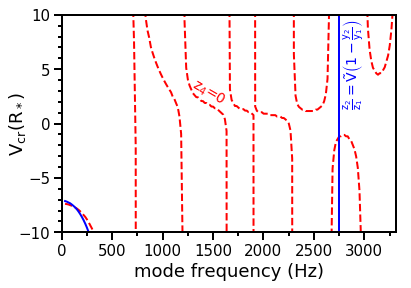
\includegraphics[width=0.45\textwidth,angle=0]{minima_30_50_-80.png}
\caption{The eigenvalues that satisfy the jump conditions at the crust-core boundary, showing the location of two modes (the crust-core interface mode and the fundamental mode). This figure uses the EOS parameterised by $J=30$ MeV, $L=50$ MeV, and $K_{\rm sym}=-80$ MeV.}
\label{fig:trace_minima}
\end{figure}


Figure \ref{fig:2i_mode} shows the radial and transverse displacements for the interface mode. It has a distinctive peak in its radial displacement at the crust-core boundary, which is what we expect because the i-mode is caused by the discontinuity between the crust and core. For this EOS, its eigenvalues are $f=134.3$ Hz and $V(R_*)=-7.72$ (as can be seen in figure \ref{fig:trace_minima}). The transverse displacement in the core is small, while in the crust it discontinuously jumps to become large. This makes the i-mode a good candidate for an RSF because more of its energy will go into deforming the crust, helping it to reach the breaking strain faster.

\begin{figure}
\centering
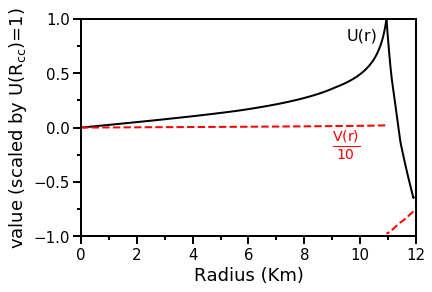
\includegraphics[width=0.45\textwidth,angle=0]{2i2_30_50_-80.png}
\caption{The quadrupole crust-core interface mode for the EOS parameterised by $J=30$ MeV, $L=50$ MeV, and $K_{\rm sym}=-80$ MeV. $V(r)$ has been reduced by an order of magnitude so that it can be plotted alongside $U(r)$.}
\label{fig:2i_mode}
\end{figure}










\section{Results}
\subsection{The Impact of Symmetry Energy Parameters on Stellar Structure} \label{sec:stellar_structure}
\hspace{\parindent}Figure \ref{fig:MR_JLK} shows the relationships between the neutron star mass and the stellar radius and crust-core transition radius, and how these relationships change as $J$, $L$ and $K_{\rm sym}$ are varied. This figure shows how the bulk properties of the star are affected by the symmetry energy parameters when holding the maximum neutron star mass ($M_{\rm max}$) and moment of inertia at $1.4 M_\odot$ ($I_{1.4}$) fixed. Within these constraints, which primarily contribute to the core EOS, $J$ has very little impact on the crust-core transition radius and a small impact on the total radius (except for low mass stars), whereas variations in $L$ and $K_{\rm sym}$ cause larger changes in both of these radii. For many different types of mode, the frequency is dependant on both the stellar radius and the crust-core transition radius, and therefore, if we only consider these three plots, we would expect mode frequencies of $1.4$ M$_{\odot}$ neutron stars to vary with $L$ and $K_{\rm sym}$ more than with $J$. However, we must also consider the impact of the symmetry energy parameters on the restoring forces that cause the modes to oscillate. For the i-mode, the restoring forces are dominated by shear forces, and therefore we would expect the impact of the symmetry energy parameters on the i-mode frequency to be closely related to their impact on the shear speed, $c_t=\sqrt{\frac{\mu}{\rho}}$. Figure \ref{fig:Mct_JLK} shows the impact of the stellar mass and the symmetry energy parameters on the density-weighted average of the shear speed. This figure shows that $J$ and $L$ have larger impacts on the average shear speed than $K_{\rm sym}$, and that the shear speed is strongly dependent on all three of the symmetry energy parameters.


By studying the trends of figures \ref{fig:MR_JLK} and \ref{fig:Mct_JLK} we can see that the symmetry energy parameters have a much larger impact on the shear speed than on the total stellar radius and the crust-core transition radius, and therefore we can predict that the symmetry energy parameters' relationships to the i-mode frequency will be similar to their relationships with the average shear speed, that is to say that $K_{\rm sym}$ will have the weakest impact on the frequency, $J$ will have a greater impact, and $L$ will have the greatest impact.





\begin{figure}
\centering
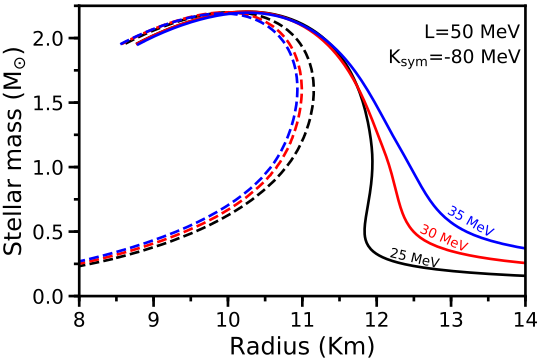
\includegraphics[width=0.45\textwidth,angle=0]{MRs_Jvals_full.png}
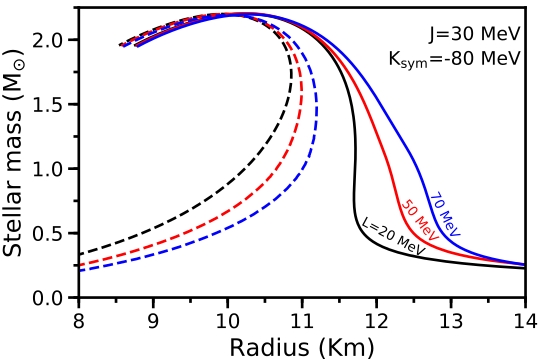
\includegraphics[width=0.45\textwidth,angle=0]{MRs_Lvals_full.png}
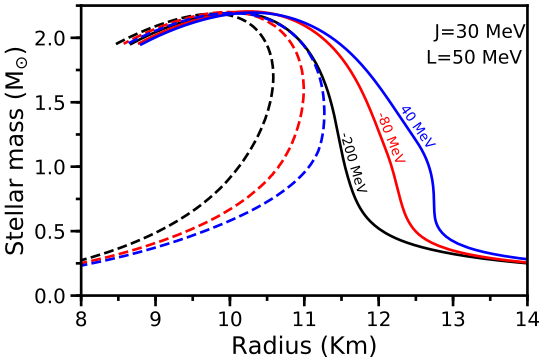
\includegraphics[width=0.45\textwidth,angle=0]{MRs_Kvals_full.png}
\caption{The relationships between the neutron star mass and the stellar radius (solid lines) and the crust-core transition radius (dashed lines) for different EOSs. Each plot varies a different symmetry energy parameter over a wide range of values, with the lines being labelled with the varied parameter. The red (middle) lines of each plot are the same.}
\label{fig:MR_JLK}
\end{figure}

% \begin{figure}
% \centering
% 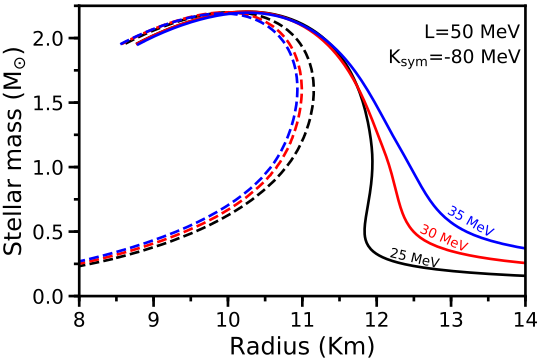
\includegraphics[width=0.45\textwidth,angle=0]{MRs_Jvals_full.png}
% \caption{The relationship between the neutron star mass and both the stellar radius (solid lines) and the location of the crust-core transition (dashed lines) for three different EOSs. These EOSs are parameterised by $L=50$ MeV, $K_{\rm sym}=-80$ MeV, and a wide range of $J$ values, with which the stellar radii are labelled.}
% \label{fig:MR_Jvals}
% \end{figure}

% \begin{figure}
% \centering
% 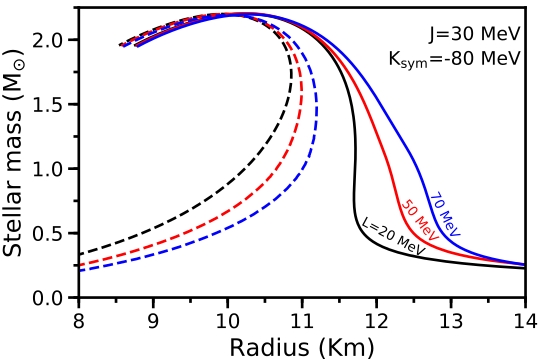
\includegraphics[width=0.45\textwidth,angle=0]{MRs_Lvals_full.png}
% \caption{The same as figure \ref{fig:MR_Jvals}, but with EOSs parameterised by a wide range of $L$ values, $J=30$ MeV and $K_{\rm sym}=-80$ MeV. The red (middle) lines are the same for both figures.}
% \label{fig:MR_Lvals}
% \end{figure}

% \begin{figure}
% \centering
% 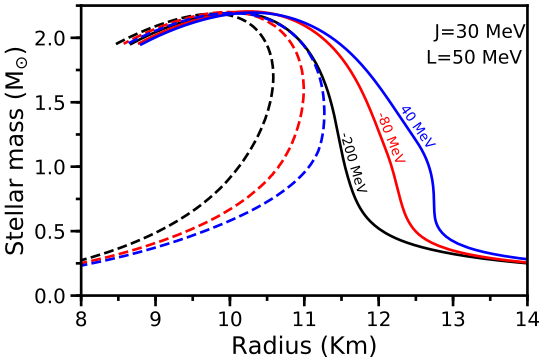
\includegraphics[width=0.45\textwidth,angle=0]{MRs_Kvals_full.png}
% \caption{The same as figure \ref{fig:MR_Jvals}, but with EOSs parameterised by a wide range of $K_{\rm sym}$ values, $J=30$ MeV and $L=50$ MeV. The red (middle) lines are the same for both figures.}
% \label{fig:MR_Kvals}
% \end{figure}


\begin{figure}
\centering
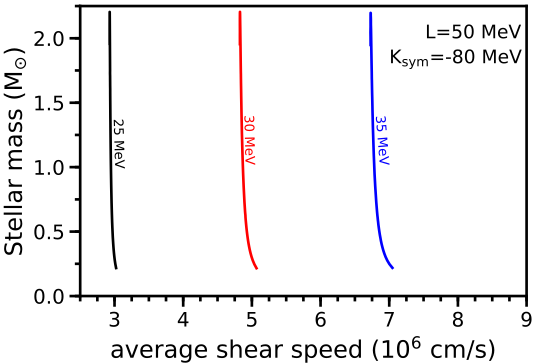
\includegraphics[width=0.45\textwidth,angle=0]{Mcts_Jvals.png}
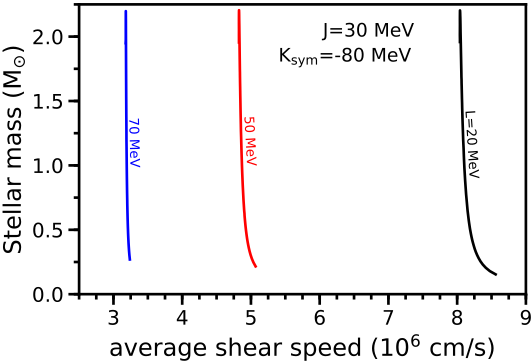
\includegraphics[width=0.45\textwidth,angle=0]{Mcts_Lvals.png}
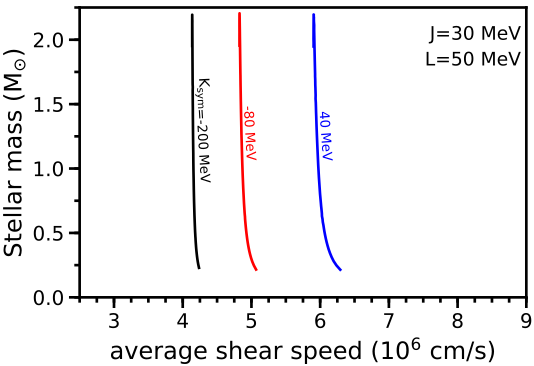
\includegraphics[width=0.45\textwidth,angle=0]{Mcts_Kvals.png}
\caption{The relationship between the neutron star mass and the density-weighted average shear speed for different EOSs. Each plot varies a different symmetry energy parameter over a wide range of values, with the lines being labelled with the varied parameter. The red (middle) lines of each plot are the same.}
\label{fig:Mct_JLK}
\end{figure}

% \begin{figure}
% \centering
% 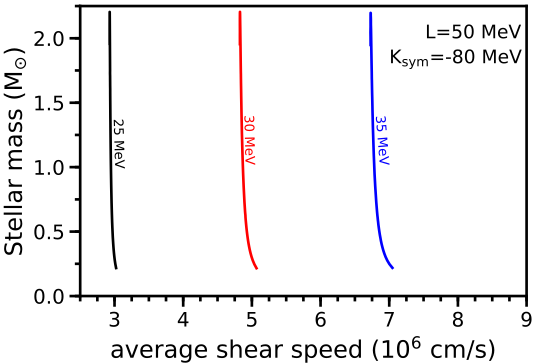
\includegraphics[width=0.45\textwidth,angle=0]{Mcts_Jvals.png}
% \caption{The relationship between the stellar mass and the density-weighted average shear speed for three different EOSs. These EOSs are parameterised by $L=50$ MeV, $K_{\rm sym}=-80$ MeV, and a wide range of $J$ values, with which the lines are labelled.}
% \label{fig:Mct_Jvals}
% \end{figure}

% \begin{figure}
% \centering
% 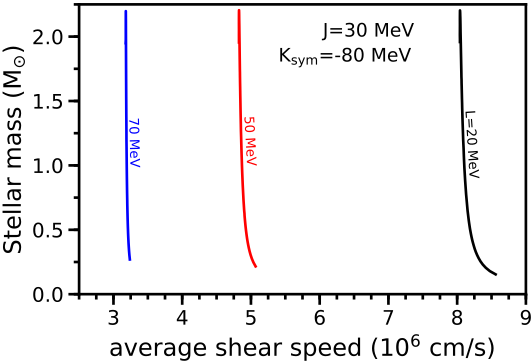
\includegraphics[width=0.45\textwidth,angle=0]{Mcts_Lvals.png}
% \caption{Similar to figure \ref{fig:Mct_Jvals}, but for EOSs parameterised by $J=30$ MeV, $K_{\rm sym}=-80$ MeV, and a wide range of $L$ values. The red (middle) lines are the same for both figures.}%Note that the EOS using J=30, L=80, K=-80 is acausal, and so we can't plot the full L range while keeping J and K in the middle of their ranges.
% \label{fig:Mct_Lvals}
% \end{figure}

% \begin{figure}
% \centering
% 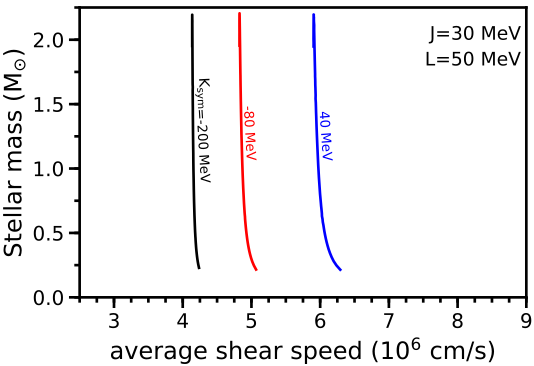
\includegraphics[width=0.45\textwidth,angle=0]{Mcts_Kvals.png}
% \caption{Similar to figure \ref{fig:Mct_Jvals}, but for EOSs parameterised by $J=30$ MeV, $L=50$ MeV, and a wide range of $K_{\rm sym}$ values. The red (middle) lines are the same for both figures.}
% \label{fig:Mct_Kvals}
% \end{figure}













\subsection{Interface Mode dependence on Nuclear Parameters}
\label{sec:EoS_sets}
\hspace{\parindent}For the remainder of this paper, unless otherwise stated, we focus our results on $M_*=1.4M_{\odot}$ neutron stars. We explored the three different ranges of symmetry energy parameters described in Section \ref{sec:nuclear_model}. In Section \ref{subsec4_1_1}, we use our uniform (weakly-constrained) $J$, $L$ and $K_{\rm sym}$ ranges, in order to avoid tying our results to those of previous works. In Section \ref{subsec4_1_2}, the ranges of the symmetry energy parameters are chosen to match the constraints determined by pure neutron matter theory, as this is the most relevant constraint for neutron star matter, which is extremely neutron rich. Finally, in Section \ref{subsec4_1_3}, we take $K_{\rm sym}$ to be a particular function of $J$ and $L$, allowing us to see the importance of uncertainty in $K_{\rm sym}$, and letting us more directly compare with previous works that have only allowed the first two symmetry energy parameters to vary, such as \citet{chen2010density}, \citet{steiner2012connecting} and \citet{tsang2009constraints}.







\subsubsection{Uniform (weakly-constrained) $J$, $L$ and $K_{\rm sym}$ range}\label{subsec4_1_1}
\hspace{\parindent} After constructing a grid of stellar models, we calculated the $\ell = 2$ i-mode frequency for each of these stars, and then interpolated between them to find surfaces of constant frequency in the weakly-constrained uniform $J$,$L$,$K_{\rm sym}$ parameter space, shown in figure \ref{fig:grid_J_L_K}.




\begin{figure}
\centering
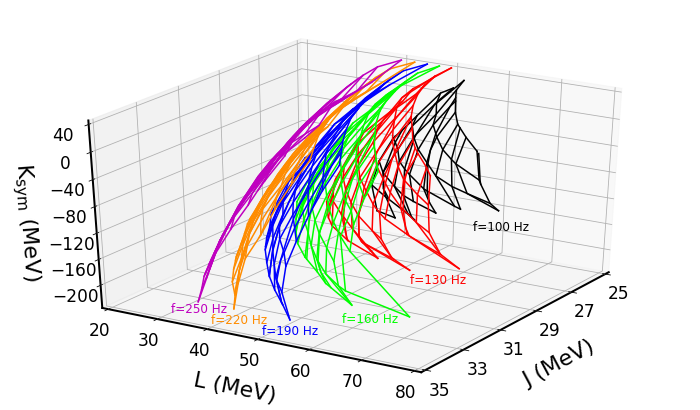
\includegraphics[width=0.45\textwidth,angle=0]{grid_J_L_K.png}
\caption{Surfaces of constant i-mode frequency in the weakly-constrained symmetry energy parameter space of our uniform distribution. The surfaces are $30$ Hz apart.}
\label{fig:grid_J_L_K}
\end{figure}

 



The relationship between frequency, $J$ and $L$ is shown in figure \ref{fig:J_vs_L_vs_f+tc} (for $K_{\rm sym}=-80$ MeV). On the right side of the plot is the time before coalescence at which the corresponding gravitational wave frequencies occur, calculated by \citep{tsang2012resonant,blanchet2006gravitational}
\begin{align}
t_c-t=\frac{3}{8}t_{GW}=1.76\times 10^{-3}\rm{s}\left(\frac{\mathcal{M}}{1.2M_{\odot}}\right)^{-\frac{5}{3}}\left(\frac{f_{GW}}{1000 \rm{Hz}}\right)^{-\frac{8}{3}},
\label{eq:t_before_merger}
\end{align}
\noindent where $\mathcal{M}=\frac{M_1^{\frac{3}{5}}M_2^{\frac{3}{5}}}{(M_1+M_2)^{\frac{1}{5}}}$ is the chirp mass and $t_c-t$ is the time before the merger. From this figure we can see that the frequency increases with increasing $J$ and decreasing $L$, and that the change over the $L$ range is greater than the change of the $J$ range, meaning that $L$ has a greater impact on the properties of the star that determine the i-mode frequency. Similarly, from figure \ref{fig:L_vs_K_vs_f+tc} we see that at low $L$ values, $K_{\rm sym}$ has a significant impact on the frequency, but as $L$ is increased, $K_{\rm sym}$'s impact decreases. Figures \ref{fig:grid_J_L_K}, \ref{fig:J_vs_L_vs_f+tc} and \ref{fig:L_vs_K_vs_f+tc} show that for a low frequency detection of an RSF, the constraints we could obtain for $L$ and $K_{\rm sym}$ would be weaker than for a higher frequency detection, while the strength of the constraint of $J$ is similar for both high and low i-mode frequencies. Note that some combinations of the symmetry energy parameters within our chosen ranges result in EOSs that are nonphysical, and therefore have been discarded. For example, we can see from figure \ref{fig:J_vs_L_vs_f+tc} that there is no EOS for $J=30$ MeV, $L=80$ MeV, $K_{\rm sym}=-80$ MeV.
%lower f = closer L lines & reduced df/dL = weaker constraint on L
%lower f = closer K lines = weaker constraint on K
%lower f = similar df/dJ = similar constraint on J


\begin{figure}
\centering
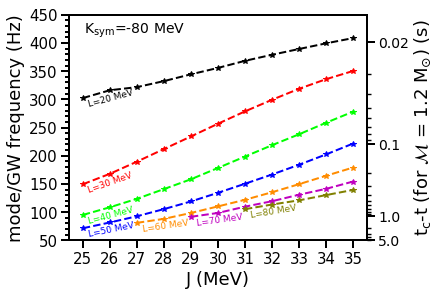
\includegraphics[width=0.45\textwidth,angle=0]{J_L_f_tc_K-80.png}
\caption{The i-mode frequency for various $J$ and $L$ values, with $K_{\rm sym}=-80$ MeV. On the right axis of the plot are the times before coalescence at which the corresponding frequencies occur. The dashed lines connect EOSs with the same $L$ values.}
\label{fig:J_vs_L_vs_f+tc}
\end{figure}


\begin{figure}
\centering
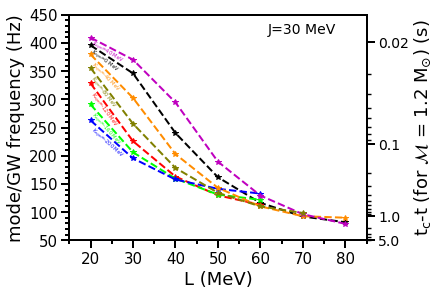
\includegraphics[width=0.45\textwidth,angle=0]{L_K_f_tc_J30.png}
\caption{The i-mode frequency for various $L$ and $K_{\rm sym}$ values, with $J=30$ MeV. On the right axis of the plot are the times before coalescence at which the corresponding frequencies occur. The dashed lines connect EOSs with the same $K_{\rm sym}$ values.}
\label{fig:L_vs_K_vs_f+tc}
\end{figure}


In order to better understand figure \ref{fig:grid_J_L_K}, we plot its two-dimensional projections, shown in figure \ref{fig:freq_contours_plane}. The first plot of this figure shows the values of $J$ and $L$ that can result in the i-mode having the chosen frequency, with the spread in $L$ at any given $J$ being due to the range of possible $K_{\rm sym}$ values. The second and third plots show the projections on $J$ and $K_{\rm sym}$, and on $L$ and $K_{\rm sym}$. However, $J$ and $L$ have much larger impacts on the i-mode frequency than $K_{\rm sym}$, and therefore the spread is much larger. In particular, the frequency is so dependent on $L$ that the chosen frequencies can be obtained from almost any combination of $J$ and $K_{\rm sym}$ (within the ranges of the symmetry energy parameters that we have used here).


\begin{figure}
\centering
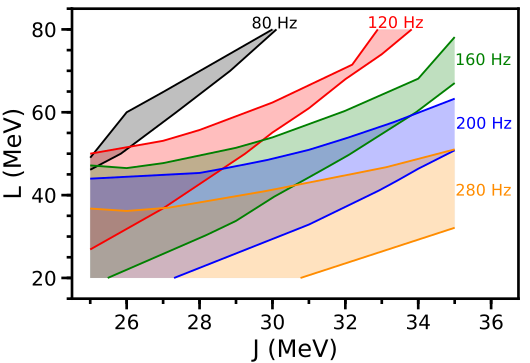
\includegraphics[width=0.45\textwidth,angle=0]{grid_JL_Kspread.png}
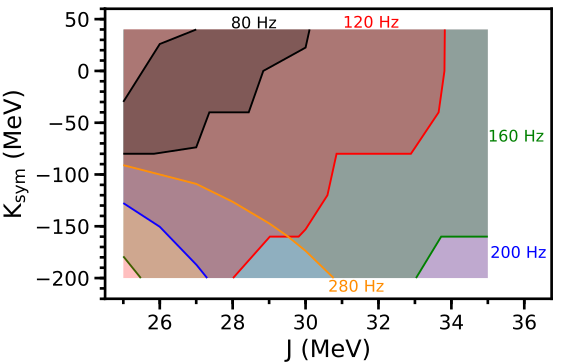
\includegraphics[width=0.45\textwidth,angle=0]{grid_JK_Lspread.png}
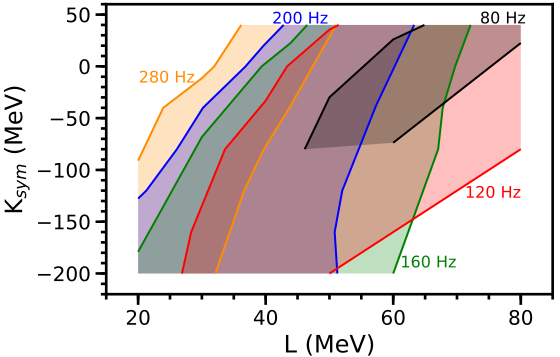
\includegraphics[width=0.45\textwidth,angle=0]{grid_LK_Jspread.png}
\caption{The 2D projections of figure \ref{fig:grid_J_L_K}, showing the ranges of the symmetry energy parameters in which five example i-mode frequencies can be obtained. The widths of the regions are caused by the ranges of the symmetry energy parameters given in Section \ref{sec:nuclear_model}.}
\label{fig:freq_contours_plane}
\end{figure}



To calculate the constraints we could place on $J$, $L$, and $K_{\rm sym}$, we need to find the sources of uncertainty in the i-mode frequency. One such uncertainty is due to the timescale over which resonant excitation of a mode can occur. This can be calculated as \citep{tsang2012resonant}
\begin{align}
t_{\rm res}\sim 8\times10^{-2}\text{s}\left(\frac{\mathcal{M}}{1.2\text{M}_{\odot}}\right)^{\frac{-5}{6}}\left(\frac{f_{\rm mode}}{100 \text{ Hz}}\right)^{\frac{-11}{6}}.
\label{eq:res_timescale}    
\end{align}
\noindent This can be combined with the rate of change of the gravitational wave frequency
\begin{align}
\Dot{f}_{\rm gw}=\frac{f_{\rm gw}}{4.7\times10^{-3}\text{s}}\left(\frac{\mathcal{M}}{1.2\text{M}_{\odot}}\right)^{\frac{5}{3}}\left(\frac{f_{\rm gw}}{1000 \text{ Hz}}\right)^{\frac{8}{3}}
\label{eq:df_GW/dt}    
\end{align}
\noindent (where $f_{\rm gw}\approx f_{\rm mode}$) to obtain a simple estimate of the range of frequencies over which resonance can occur:
\begin{align}
\delta f\sim t_{\rm res}\Dot{f}_{\rm gw}\sim3.7\text{Hz}\left(\frac{\mathcal{M}}{1.2\text{M}_{\odot}}\right)^{\frac{5}{6}}\left(\frac{f_{\rm mode}}{100 \text{ Hz}}\right)^{\frac{11}{6}}.
\label{eq:freq_spread}    
\end{align}
\noindent From this we see that the resonance window gets larger as the frequency increases, with $\delta f$ scaling as $f_{\rm mode}^{\frac{11}{6}}$. For a chirp mass of $1.2M_{\odot}$ and a resonance at $100$ Hz, we get a frequency range of $\delta f\sim 3.7$ Hz, and for a resonance at $160$ Hz we get a range of $\delta f\sim 8.8$ Hz. This means that the spread of the frequency contours in the $J,L$ plane (seen in figure \ref{fig:t_res_spread}) is quite small ($\delta L\lesssim 5$ MeV), and therefore the impact of the resonance window is significantly less than that of the $K_{\rm sym}$ range, which causes a spread of $\sim 20$ MeV in $L$ at any given $J$ value. It should be noted that this is a very conservative estimate, and that by more accurately calculating both the rate at which energy is transferred into the modes and the breaking strain of the crust, this uncertainty could be significantly reduced by calculating the time it takes for the crust to shatter.

\begin{figure}
\centering
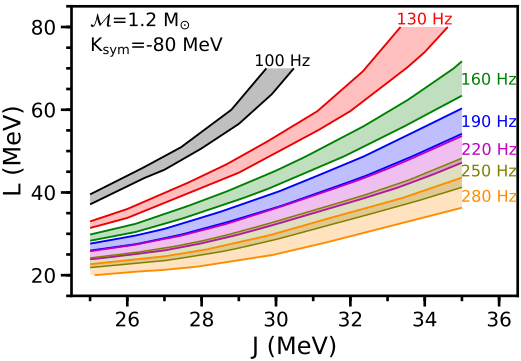
\includegraphics[width=0.45\textwidth,angle=0]{JL_dfspread.png}
\caption{The spread in the frequency contours in the $J$,$L$ plane for a particular $K_{\rm sym}$ value, if we consider that the i-mode frequency can be anywhere within the resonance window (ie: the i-mode frequency can have any value between $f_{GW}-\delta f$ and $f_{GW}+\delta f$).}
\label{fig:t_res_spread}
\end{figure}


In figure \ref{fig:all_constraints} we plot the regions in $J$,$L$ that can give certain chosen frequencies when considering both the $K_{\rm sym}$ range (figure \ref{fig:freq_contours_plane}) and the resonance window (figure \ref{fig:t_res_spread}), and compare it to the combined experimental nuclear constraints given in \citet{lattimer2013constraining} (which includes constrains from: fits to nuclear masses \citep{kortelainen2010nuclear}, neutron skin thickness \citep{chen2010density}, dipole polarisability \citep{piekarewicz2012electric}, giant dipole resonances \citep{trippa2008giant}, and isotope diffusion in heavy ion collisions \citep{tsang2009constraints}). From these results, in order to agree with the combined experimental nuclear constraints, we could expect to observe precursor flares at $f_{GW}=150^{+130}_{-30}$ Hz. The range is very large because this figure shows the most conservative estimate of our $J$,$L$ constraints, with the upper bounds using $f\rightarrow f-\delta f$ Hz and $K_{\rm sym}=40$ MeV, and the lower bounds using $f\rightarrow f+\delta f$ Hz and $K_{\rm sym}=-200$ MeV. We could also plot the regions in $J$,$K_{\rm sym}$ and $L$,$K_{\rm sym}$ that give the chosen frequencies, but we find that the strong dependence of the frequency on $J$ and $L$ means that these plots are uninformative. Therefore, in order to find more useful constraints, we constrain the initial ranges of $J$, $L$ and $K_{\rm sym}$ used to generate the EOSs.

\begin{figure}
\centering
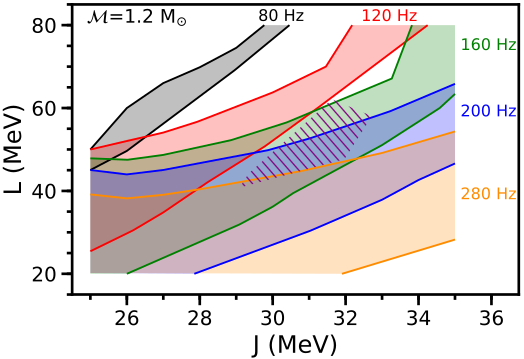
\includegraphics[width=0.45\textwidth,angle=0]{grid_JL_Kdfspread_2.png}
\caption{The constraints we could apply to $J$ and $L$, assuming that the value of $K_{\rm sym}$ can be anywhere in the range $-200$ to $40$ MeV at all $J$ and $L$ values, and that the uncertainty in the i-mode frequency due to the resonance window is given by equation \ref{eq:freq_spread}. The hatched area in the centre of the plot represents the combined experimental nuclear constraints on $J$ and $L$ \citep{lattimer2013constraining}.}
\label{fig:all_constraints}
\end{figure}









\subsubsection{$J$, $L$ and $K_{\rm sym}$ constrained using pure neutron matter theory (PNM) } \label{subsec4_1_2}

\noindent Using a set of EOSs consistent with the results of pure neutron matter theory (the PNM priors of \citet{newton2020nuclear}, see section \ref{sec:nuclear_model}), we calculate the i-mode frequencies to obtain surfaces in the $J$,$L$,$K_{\rm sym}$ parameter space on which the frequency is constant, shown in figure \ref{fig:PNM_planes}. 

\begin{figure}
\centering
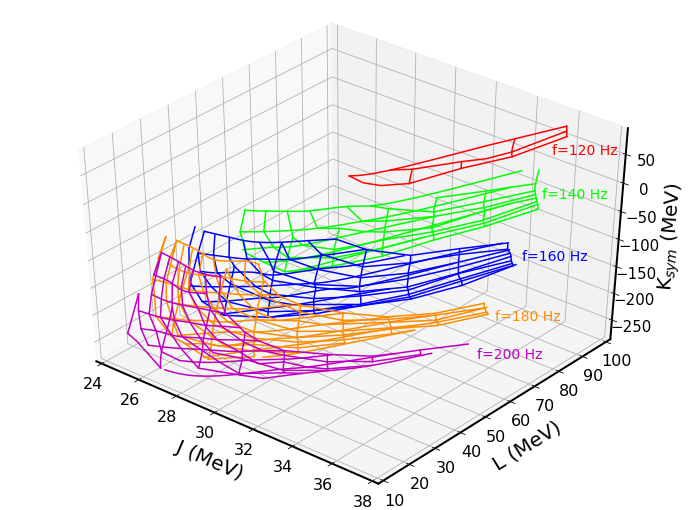
\includegraphics[width=0.45\textwidth,angle=0]{PNM_planes}
\caption{Surfaces of constant i-mode frequency in the $J$,$L$,$K_{\rm sym}$ parameter space, where the $J$, $L$ and $K_{\rm sym}$ ranges are constrained by pure neutron matter theory. The surfaces are 20 Hz apart.}
\label{fig:PNM_planes}
\end{figure}

Similar to figure \ref{fig:freq_contours_plane}, figure \ref{fig:PNM_2d} shows two-dimensional projections of figure \ref{fig:PNM_planes}. In the first plot, for a given frequency, having a wider range in $L$ at a particular $J$ value means that the possible range of $K_{\rm sym}$ values has a greater impact on the i-mode frequency. We can see that $K_{\rm sym}$ has a small impact on the i-mode frequency, particularly at higher $J$ values. We can also see (from the high spread in $K_{\rm sym}$ on the other two plots) that $L$ and $J$ both have large impacts on the i-mode frequency. However, the prior ranges of the symmetry energy parameters are much smaller than in Section \ref{subsec4_1_1}, and by comparing figures \ref{fig:PNM_2d} and \ref{fig:freq_contours_plane} we can see that this significantly reduces the ranges of the symmetry energy parameters that can be used to obtain a chosen frequency.

\begin{figure}
\centering
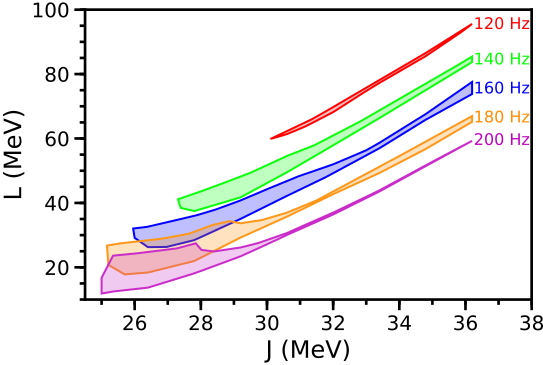
\includegraphics[width=0.45\textwidth,angle=0]{PNM_JL}
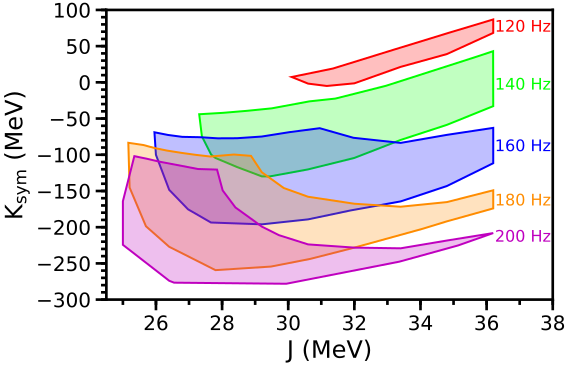
\includegraphics[width=0.45\textwidth,angle=0]{PNM_JK}
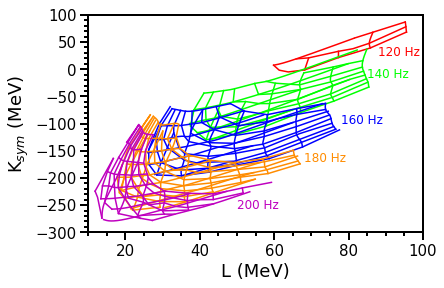
\includegraphics[width=0.45\textwidth,angle=0]{PNM_LK}
\caption{The 2D projections of figure \ref{fig:PNM_planes}, showing the ranges of the symmetry energy parameters in which five example i-mode frequencies can be obtained while being consistent with pure neutron matter theory.}
\label{fig:PNM_2d}
\end{figure}

To calculate the constraint that could be placed on $J$ and $L$, we calculate the resonance window using equation \ref{eq:freq_spread}. This, combined with the $K_{\rm sym}$ range, results in figure \ref{fig:PNM_JL_res_spread}, which shows the constraint we could apply to $J$ and $L$ for five different frequencies alongside the combined nuclear physics constraints from \citet{lattimer2013constraining}. By comparing figures \ref{fig:PNM_JL_res_spread} and \ref{fig:all_constraints}, we can see that requiring consistency with pure neutron matter theory has significantly tightened our constraints, with $f_{GW}=150^{+30}_{-30}$ Hz agreeing with the combined experimental nuclear constraints. 



\begin{figure}
\centering
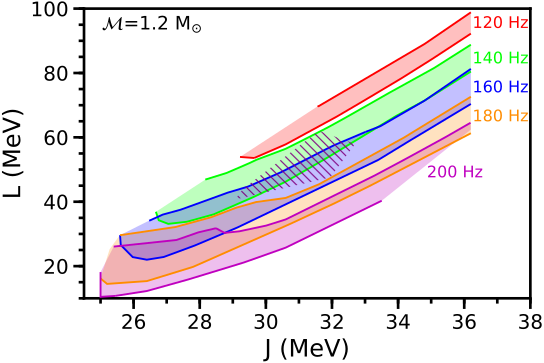
\includegraphics[width=0.45\textwidth,angle=0]{PNM_JL_Kdfspread_2.png}
\caption{The constraints that we could apply to $J$ and $L$ in the event of an RSF detection at different frequencies, with the strength of each constraint being determined by the $K_{\rm sym}$ range and the width of the resonance window, where the $J$, $L$ and $K_{\rm sym}$ ranges are constrained by pure neutron matter theory. The hatched area in the centre of the plot indicates the combined experimental nuclear constraints on $J$ and $L$.}
\label{fig:PNM_JL_res_spread}
\end{figure}

As the $J$ and $L$ ranges are smaller than in Section \ref{subsec4_1_1}, the constraints that we could apply to $J$,$K_{\rm sym}$ and $L$,$K_{\rm sym}$ are much tighter. In figure \ref{fig:PNM_JK_res_spread} (\ref{fig:PNM_LK_res_spread}) we have plotted the constraint that could be applied to $J$ and $K_{\rm sym}$ ($L$ and $K_{\rm sym}$) due to an RSF detection, with the strength of the constraint being determined by the $L$ ($J$) range and the width of the resonance window.

\begin{figure}
\centering
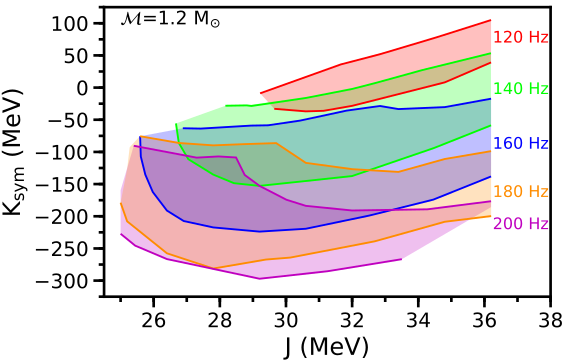
\includegraphics[width=0.45\textwidth,angle=0]{PNM_JK_Ldfspread.png}
\caption{Similar to figure \ref{fig:PNM_JL_res_spread}, but for the constraint that could be applied to $J$ and $K_{\rm sym}$, with the strength of the constraint being determined by the $L$ range and the width of the resonance window.}
\label{fig:PNM_JK_res_spread}
\end{figure}

\begin{figure}
\centering
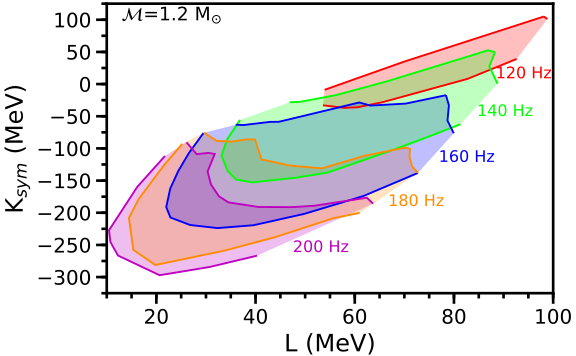
\includegraphics[width=0.45\textwidth,angle=0]{PNM_LK_Jdfspread.png}
\caption{Similar to figure \ref{fig:PNM_JL_res_spread}, but for the constraint that could be applied to $L$ and $K_{\rm sym}$, with the strength of the constraint being determined by the $J$ range and the width of the resonance window.}
\label{fig:PNM_LK_res_spread}
\end{figure}











\subsubsection{K$_{\rm sym}$ as a function of J and L (MSL0)}\label{subsec4_1_3}
\hspace{\parindent}Using the MSL0 model for the $K_{\rm sym}$ dependence on $J$ and $L$, as an example of a more restricted two-parameter Skyrme model, we calculated the i-mode frequencies for a grid of $J$ and $L$ values to obtain figure \ref{fig:MSL0_J_L_f_tc}.

\begin{figure}
\centering
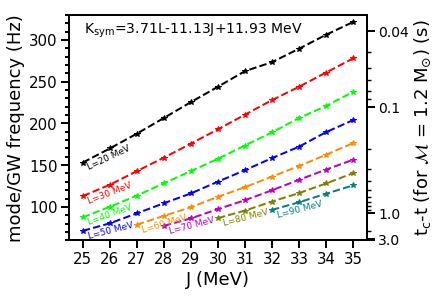
\includegraphics[width=0.45\textwidth,angle=0]{MSL0_J_L_f_tc}
\caption{The relationship between $J$, $L$ and the i-mode frequency with the MSL0-like $K_{\rm sym}$ dependence. As there is no $K_{\rm sym}$ range, this plot shows every EOS that we used in Section \ref{subsec4_1_3}.}
\label{fig:MSL0_J_L_f_tc}
\end{figure}

Next we interpolated between the EOSs to obtain frequency contours in the $J$,$L$ plane, shown in figure \ref{fig:MSL0_contours_20gap}. Now that $K_{\rm sym}$ is not a free parameter, the contours in the $J$,$L$ plane are only spread by the resonance window (equation \ref{eq:freq_spread}), giving us figure \ref{fig:MSL0_shaded_constraints}, where we have also plotted the nuclear physics constraints on $J$ and $L$. These results represent a best case scenario for the $K_{\rm sym}$ range, as there is no uncertainty in its value at all $J$ and $L$ values. From this figure we can see that a precursor flare detected at a gravitational wave frequency of $f_{GW}=140^{+40}_{-20}$ Hz would provide $J$,$L$ constraints that agree with those from nuclear physics. 

\begin{figure}
\centering
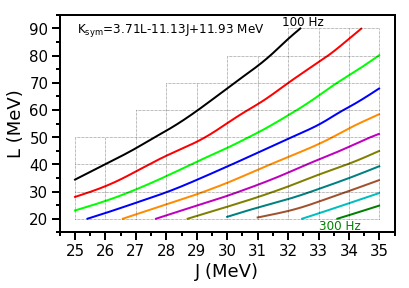
\includegraphics[width=0.45\textwidth,angle=0]{MSL0_contours_20gap}
\caption{Frequency contours in the $J$,$L$ plane with the MSL0-like $K_{\rm sym}$ dependence. The contours are $20$ Hz apart. The grid in the background indicates the $J$ and $L$ values of the EOSs that we interpolated between.}
\label{fig:MSL0_contours_20gap}
\end{figure}

\begin{figure}
\centering
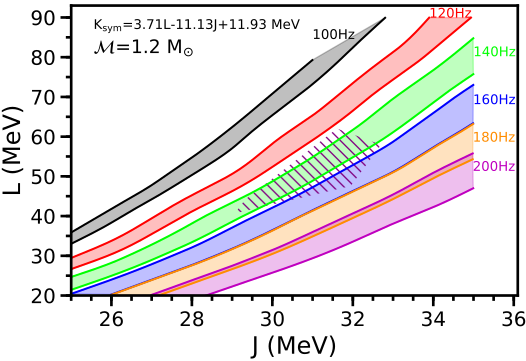
\includegraphics[width=0.45\textwidth,angle=0]{MSL0_JL_Kdfspread_2.png}
\caption{Frequency contours in the $J$,$L$ plane that have been spread by the resonance window (with the MSL0-like $K_{\rm sym}$ dependence). The hatched area in the centre of the plot indicates the combined experimental nuclear constraints on $J$ and $L$.}
\label{fig:MSL0_shaded_constraints}
\end{figure}









\begin{table}
\centering
\begin{tabular}{|c|c|}
\hline
$J$, $L$, $K_{\rm sym}$ ranges&GW frequency of the RSF (Hz)\\

\hline
$ $& $ $\\[-9pt]
Uniform&$150^{+130}_{-30}$\\
\hline
$ $& $ $\\[-9pt]
PNM&$150^{+30}_{-30}$\\
\hline
$ $& $ $\\[-9pt]
MSL0&$140^{+40}_{-20}$\\
\hline
\end{tabular}
\caption{Summary of, for each of our data sets, the gravitational wave frequency at which a Resonant Shattering Flare needs to occur in order to agree with the combined experimental nuclear constraints on $J$ and $L$ given in \citet{lattimer2013constraining}. These results are for the Skyrme model described in \citet{newton2020nuclear}, using Newtonian perturbations and a $M_*=1.4$ M${_\odot}$ neutron star.}
\label{tab:freq_to_match_nuclear}
\end{table}

Table \ref{tab:freq_to_match_nuclear} inverts our method for constraining the symmetry energy parameters by showing the gravitational wave frequencies at which we would expect to observe a RSF in order to agree with experimental constraints on $J$ and $L$ \citep{lattimer2013constraining}. From this we can see that, for the model used in this work and a $1.4$ M$_{\odot}$ neutron star, we expect to observe RSFs at gravitational wave frequencies of around $150$ Hz, or approximately $0.3$ s before coalescence.









\subsection{Shear speed}

\hspace{\parindent}In order determine the cause of the change in frequency due to changes in $J$, $L$ and $K_{\rm sym}$, we investigated how the properties of the star change with $J$, $L$ and $K_{\rm sym}$. As we predicted in section \ref{sec:stellar_structure}, the density-weighted average of the shear speed in the crust was closely related to the i-mode frequency. Figure \ref{fig:f_avct_MSL0} relates the frequency and the average shear speed for each of EOSs that we have used in this work.


\begin{figure}
\centering
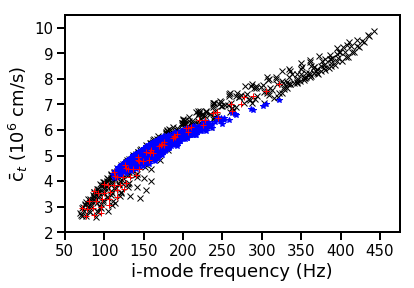
\includegraphics[width=0.45\textwidth,angle=0]{f_vs_avct_grid_PNM_MSL0.png}
\caption{The relationship between the i-mode frequency and the density-weighted average shear speed for each of our EOSs. The EOSs in black use the weakly constrained $J$, $L$ and $K_{\rm sym}$ ranges, the EOSs in blue use symmetry energy parameters that are consistent with pure neutron matter theory, and the EOSs in red use the MSL0-like $K_{\rm sym}$ dependence.}
\label{fig:f_avct_MSL0}
\end{figure}

In a similar way to how we obtained frequency contours in the $J$,$L$ plane, we can obtain average shear speed contours. This is shown in figure \ref{fig:avct_JL_MSL0} for the EOSs with the MSL0-like $K_{\rm sym}$ dependence, and from this we can see that these contours are similar to the frequency contours shown in figure \ref{fig:MSL0_contours_20gap}. However, the contours in these two plots become less similar at higher $J$ and $L$ values, meaning that properties other than the average shear speed become more significant at those values. We can also use the EOSs with weakly constrained symmetry energy parameters, and those constrained by PNM theory, to find the spread in the average shear speed contours in the $J$,$L$ plane due to $K_{\rm sym}$. This can be seen in figures \ref{fig:avct_JL_grid} and \ref{fig:avct_JL_PNM}

\begin{figure}
\centering
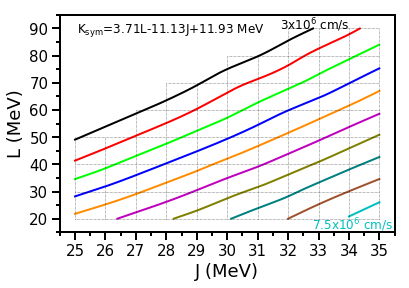
\includegraphics[width=0.45\textwidth,angle=0]{avct_contours.png}
\caption{Similar to figure \ref{fig:MSL0_contours_20gap}, but for contours in the density-weighted average shear speed. This figure is for EOSs that use the MSL0-like $K_{\rm sym}$ dependence, and the contours are separated by $5\times 10^5$ cm/s.}
\label{fig:avct_JL_MSL0}
\end{figure}

\begin{figure}
\centering
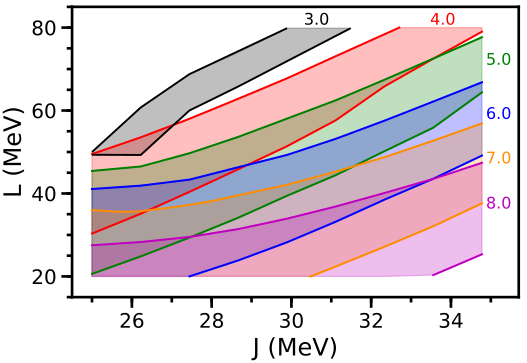
\includegraphics[width=0.45\textwidth,angle=0]{avct_grid_Kspread.png}
\caption{Similar to figure \ref{fig:all_constraints}, but for the density-weighted average shear speed. The spread is due to the weakly constrained $K_{\rm sym}$ range, and the regions are labelled in $10^6 \rm{cm/s}$.}
\label{fig:avct_JL_grid}
\end{figure}

\begin{figure}
\centering
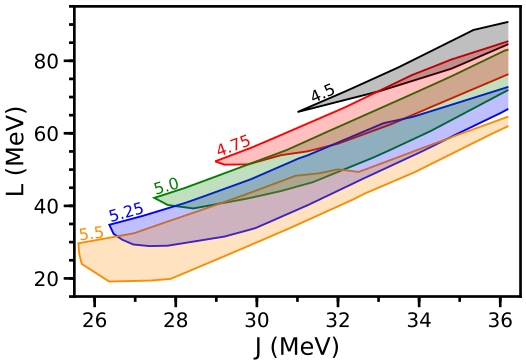
\includegraphics[width=0.45\textwidth,angle=0]{PNM_avct_JL_Kspread.png}
\caption{Similar to figure \ref{fig:PNM_JL_res_spread}, but for the density-weighted average shear speed. The spread is due to the $K_{\rm sym}$ range, which is consistent with pure neutron matter theory, and the regions are labelled in $10^6 \rm{cm/s}$.}
\label{fig:avct_JL_PNM}
\end{figure}



\section{Discussion}
\hspace{\parindent}We have calculated the relationship between the neutron star interface mode frequency and the first three parameters that characterise the density dependence of the nuclear symmetry energy at saturation density $J$, $L$ and $K_{\rm sym}$ within extended Skyrme mean-field model for the crust and outer core supplemented by two polytropes to control for the high density EoS. We have used this to present potential constraints on the symmetry energy and its derivatives that could be obtained by coincident multimessenger detection of a Resonant Shattering Flare during a NS merger. These constraints have been shown to be competitive with current nuclear experimental constraints.

Previous works have shown \citep{abbott2017gw170817,de2018tidal,abbott2018gw170817} that the gravitational wave chirp with sufficient signal-to-noise ratio can constrain the tidal deformability, total mass, and total radius. These, in turn, place constraints on the neutron star equation of state \citep{annala2018gravitational,lim2018neutron} primarily in the core. In this work, we examine the nuclear physics constraints (in particular on the nuclear symmetry energy parameters $J$, $L$, and $K_{\rm sym}$) that can be obtained by a future detection of a Resonant Shattering Flare along with a gravitational-wave chirp. Timing of the RSF relative to the GW chirp can provide a direct measurement of the resonant frequency of the $\ell = 2$ core-crust interface mode  \citep{tsang2012resonant}. This frequency is dependent on properties of the neutron star near the core-crust boundary, and is thus sensitive to the nuclear symmetry energy parameters which determine (in a model dependent way), the properties of the neutron star near nuclear saturation. The measurement of an i-mode frequency through coincident timing of an RSF would provide astrophyiscal constraints orthogonal to those sensitive mainly to the core EOS. 

We constructed three sets of equations of state parameterised by a grid of $J$, $L$ and $K_{\rm sym}$ values following \citet{newton2020nuclear}, while fixing the high density EoS parameters by choosing a reasonable value for $M_{\rm max}$ and the moment of inertia of a 1.4M$_{\rm odot}$ star, $I_{1.4}$. Solving for the i-mode frequencies, we were able to determine the regions in the $J$, $L$, $K_{\rm sym}$ parameter space that are constrained given measurements of different i-mode frequency values. 

For all three sets of EOSs, our constraints on $J$ and $L$ were angled in the same direction as the combined constraints from other works \citep{lattimer2013constraining}, and therefore a detection of an RSF at a frequency in the middle of the range that agrees with these constraints would provide a small improvement to our knowledge of $J$ and $L$. However, if an RSF were to be detected at a higher or lower frequency our constraints could be more interesting because their overlap with the combined experimental nuclear constraints would be much smaller.




In Figure \ref{fig:f_avct_MSL0} we showed that the i-mode frequency (a global property of the NS) is strongly dependent on the average (density-weighted) shear speed within the crust (a local material property of the crust). Therefore, the dependence of the frequency on the symmetry energy parameters is dominated by their effects on the shear modulus within the crust, and in particular near the crust-core boundary. Figures \ref{fig:avct_JL_MSL0}, \ref{fig:avct_JL_grid} and \ref{fig:avct_JL_PNM} relate the shear speed to the symmetry energy parameters $J$ and $L$ \citep[similar to Figure 1 of ][]{steiner2009constraints}, connecting changes in these nuclear physics parameters to their impact on the average shear speed in the neutron star crust. While other global properties of the stellar structure (e.g. neutron star radius, radius of the core-crust transition) which vary with the model parameters ($J$, $L$, $K_{\rm sym}$, $M_{\rm max}$ and $I_{1.4}$) also play a role, we find that the i-mode frequency depends most strongly on the average shear speed, as can be seem from the similarities between figures \ref{fig:avct_JL_MSL0}, \ref{fig:avct_JL_grid} and \ref{fig:avct_JL_PNM} and figures \ref{fig:MSL0_contours_20gap}, \ref{fig:all_constraints} and \ref{fig:PNM_JL_res_spread}.


The shear speed increasing with $J$ and $K_{\rm sym}$ and decreasing with $L$ is correlated with the impact of these changes on the symmetry energy in the crust (where $n_{\rm b}<n_0$); increasing $J$ and $K_{\rm sym}$ and decreasing $L$ causes the symmetry energy at crustal densities to increase, as can be seen in figure \ref{fig:Esym_JLK} (where a typical crust-core transition density is indicated by the vertical dotted line). Increasing the symmetry energy increases the energy cost of creating more neutrons, and therefore decreases the fraction of dripped neutrons in the crust. Equation~(\ref{eq:neutrons_ions}) shows that as the dripped neutron fraction decreases, the ion number density increases for a fixed mass number of nucleus in the crust. This leads to an increase in the shear modulus, as can be seen in equations~(\ref{eq:mu_1991_a}) or~(\ref{eq:altmu}). By calculating the density-averaged neutron fraction $\bar{X}_{\rm n}$, mass number $\bar{A}$ and charge number $\bar{Z}$ we have confirmed that changes in $\bar{X}_{\rm n}$ are the dominant outcome of varying any of the three symmetry energy parameters. 

Together, figures \ref{fig:Esym_JLK}, \ref{fig:f_avct_MSL0}, provide a qualitative physical understanding of the i-mode frequency dependence shown in Figures \ref{fig:all_constraints}, \ref{fig:PNM_JL_res_spread}, and \ref{fig:MSL0_shaded_constraints}. The symmetry energy profile of the star determines the composition and shear modulus in the inner crust, on which the i-mode frequency is strongly dependent.



\begin{figure}
\centering
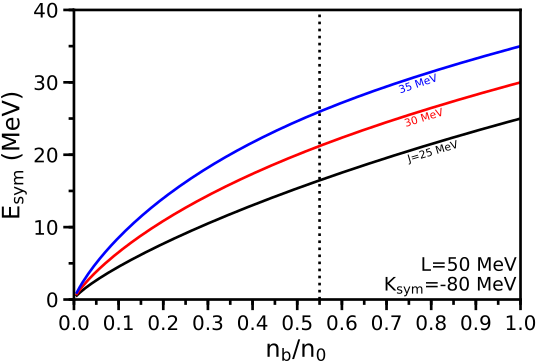
\includegraphics[width=0.45\textwidth,angle=0]{Esym_nb_J.png}
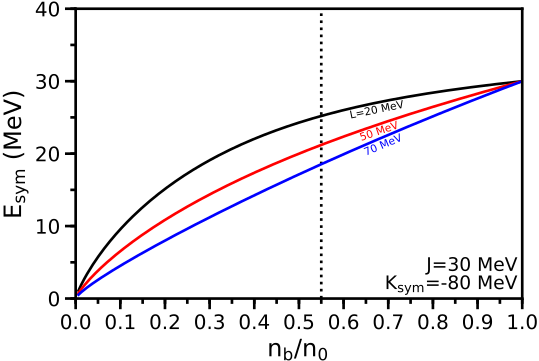
\includegraphics[width=0.45\textwidth,angle=0]{Esym_nb_L.png}
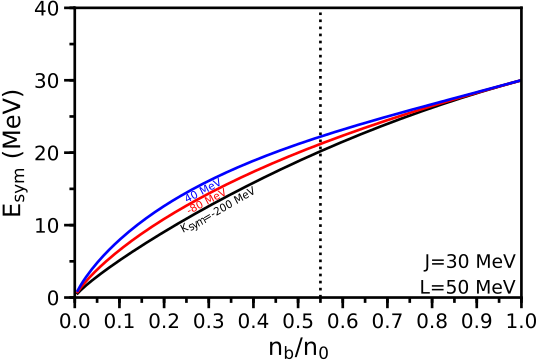
\includegraphics[width=0.45\textwidth,angle=0]{Esym_nb_K.png}
\caption{The symmetry energy below nuclear saturation density for different combinations of symmetry energy parameters. Each plot varies a different parameter over a wide range of values, with the lines being labelled with the varied parameter. The dotted line indicates the (approximate) crust-core transition density. The red (middle) lines of each plot are the same.}
\label{fig:Esym_JLK}
\end{figure}







Assuming multimessenger coincident timing of a RSF, and determination of the i-mode frequency to a precision roughly determined by the duration of the flare, a conservative assumption of nuclear parameters consistent with pure neutron matter theory results provides constraints on $J$, $L$, and $K_{\rm sym}$ that are competitive with \citet{kortelainen2010nuclear}, \citet{chen2010density} and \citet{tsang2009constraints}. If we instead use a specific $K_{\rm sym}$ dependence, our results can provide significantly tighter constraints on $J$ and $L$ than these experimental results. Conversely, we can use the constraints found by other works to obtain the range of frequencies at which we would expect to observe a RSF for a $1.4$ M$_{\odot}$ neutron star. This is shown in table \ref{tab:freq_to_match_nuclear}, with the expected frequency being $\sim 120-180$ Hz.


The quantitative results presented in this work are model dependant. We have used an extended Skyrme model, in which the maximum neutron star mass was chosen to be $2.2$ M$_{\odot}$, and the moment of inertia was assumed to be in the middle of the possible range, as the aim of this study was to determine how well an RSF detection could provide additional constraints to the symmetry energy parameters. 
Using different core EOS models may result in significantly different frequencies, with \citet{tsang2012resonant} showing i-mode frequencies as low as $30$ Hz. Within the range of EoSs used here, however, the dependence of the interface modes on the crust thickness and radius appears weaker than the dependence on the crust composition. We also note that the same event that results in a coincident detection of an RSF can be used to extract the tidal deformability, whose constraints on the core EoS compliment the constraints explored here, with the added restriction that neutron star masses and EoSs are the same in the description of each phenomenon. 

It is also important to note that~\ref{eq:mu_1991_a} is a fit to calculations of the shear modulus for an ionic lattice with no dripped neutrons and ionic separations typical of the outer crust. The shear modulus of the deep inner crust, including the nuclear pasta layers \citep{Pethick:1998aa}, remains an important outstanding problem the result of which might significantly affect our results. However, the fact that the shear modulus depends on the ion separation, which in turn depends on the fraction of dripped neutrons, means that the sensitivity of the interface mode frequency to the symmetry energy is likely to persist.



%However, we have shown that the RSF constraints are complementary to those primarily sensitive to core properties. 


We have assumed a neutron star mass of $1.4$ M$_{\odot}$, but from figure \ref{fig:vary_mass_contours} we can see that a realistic degree of uncertainty in the stellar mass \citep{abbott2017gw170817} has a noticeable impact on the i-mode frequency. Therefore, uncertainty in the mass of the source of a detected RSF will widen our constraints, with its impact being similar to that of the resonance window. 

In this work we have used non-relativistic perturbations to obtain the wave-equation. The fully relativistic perturbations derived in \citet{yoshida2002nonradial} can result in 10\% changes in the mode frequencies, which is significant when compared to the width of our constraints on $J$ and $L$, and so we will explore this effect on the constraints in a future work. We have worked within the Cowling approximation \citep{cowling1941non}, ignoring perturbations of the gravitational potential. 

Accurately calculating the Schwarzschild discriminant is not simple, and as it has little impact on the i-mode we have set it to zero (i.e. we have assumed the star is barotropic). We have also assumed that the binary lifetime is much longer than the neutron stars' spin-down and cooling timescales, and so we have ignored rotational and high temperature effects. Finally, we have not considered the impact of superfluidity in the core of a neutron star. Superfluidity allows protons and neutrons to move somewhat independently of each-other, introducing a new set of counter-moving normal modes \citep{andersson2001dynamics}, as well as modifying the frequency of modes that mainly oscillate within the core of the star.


\begin{figure}
\centering
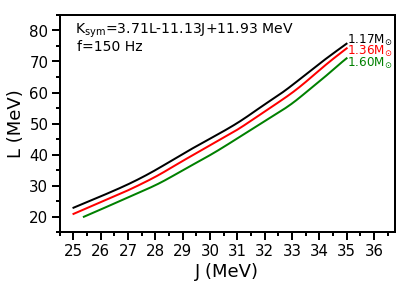
\includegraphics[width=0.45\textwidth,angle=0]{vary_mass_MSL0.png}
\caption{The effect of changing the total NS mass on the symmetry energy parameters that give a frequency of $150$ Hz, where $K_{\rm sym}$ has the MSL0-like dependence on $J$ and $L$. These mass values are the ranges calculated by \citet{abbott2017gw170817} for the stars in GW170817 (using low-spin priors).}
\label{fig:vary_mass_contours}
\end{figure}


A number of upcoming nuclear experiments promise to constrain the symmetry energy further. We highlight the ongoing efforts to extract the neutron skin of neutron rich nuclei from measurements of the parity-violating asymmetry in the electron scattering cross-section caused by the weak interaction \citep{Abrahamyan:2012aa} at Jefferson Lab and Mainz Superconducting Accelerator \citep{Horowitz:2014aa,Becker:2018aa,Thiel:2019aa}. As illustrated in figure 1 of \citet{steiner2009constraints}, neutron skins provide a constraint on the symmetry energy that is orthogonal to those provided by the constraints on the shear speed and hence the i-mode frequency. Powerful constraints may be obtained in the future by combining these weak, EM and gravitational-wave observations to probe the strong force in multi-messenger nuclear astrophysics.

Using upcoming LIGO/Virgo/KAGRA observing runs \citep{abbott2020prospects}, and existing Gamma-ray burst monitors such as Swift/BAT \citep{barthelmy2005burst} and Fermi/GBM \citep{meegan2009fermi} to provide coincident timing, the detection of a Resonant Shattering Flare from a neutron star merger can provide a new complementary astrophysical constraints on nuclear physics parameters by probing the bulk properties of neutron star matter near the crust/core transition. The rates of RSFs are currently uncertain, with precursor flares estimated to occur for $\sim3-10$\% of SGRBs. However, the recent coincident detection of a (off-axis) SGRB and the chirp from GW170817 suggests a rate of NS mergers such that we may soon be able to obtain these powerful constraints.  

\section*{Acknowledgements}

% The Acknowledgements section is not numbered. Here you can thank helpful
% colleagues, acknowledge funding agencies, telescopes and facilities used etc.
% Try to keep it short.

% %%%%%%%%%%%%%%%%%%%%%%%%%%%%%%%%%%%%%%%%%%%%%%%%%%
\section*{Data Availability}
The code to calculate the stellar models and i-mode frequencies, along with the tabulated EOSs and compositions used for the grids of symmetry energy parameters are provided i n†

%%%%%%%%%%%%%%%%%%%% REFERENCES %%%%%%%%%%%%%%%%%%

% The best way to enter references is to use BibTeX:

\bibliographystyle{mnras}
\bibliography{RSFSymmetry,newton} % if your bibtex file is called example.bib


% Alternatively you could enter them by hand, like this:
% This method is tedious and prone to error if you have lots of references
%\begin{thebibliography}{99}
%\bibitem[\protect\citeauthoryear{Author}{2012}]{Author2012}
%Author A.~N., 2013, Journal of Improbable Astronomy, 1, 1
%\bibitem[\protect\citeauthoryear{Others}{2013}]{Others2013}
%Others S., 2012, Journal of Interesting Stuff, 17, 198
%\end{thebibliography}

%%%%%%%%%%%%%%%%%%%%%%%%%%%%%%%%%%%%%%%%%%%%%%%%%%

%%%%%%%%%%%%%%%%% APPENDICES %%%%%%%%%%%%%%%%%%%%%

%\appendix
%
%\section{Some extra material}
%
%If you want to present additional material which would interrupt the flow of the main paper,
%it can be placed in an Appendix which appears after the list of references.

%%%%%%%%%%%%%%%%%%%%%%%%%%%%%%%%%%%%%%%%%%%%%%%%%%


% Don't change these lines
\bsp	% typesetting comment
\label{lastpage}
\end{document}

% End of mnras_template.tex
